\documentclass[a4paper,10pt]{extarticle}
\usepackage[ngerman]{babel}
\usepackage{amsmath,amsthm}
\usepackage{ascii}
\usepackage[adobe-utopia]{mathdesign}
\usepackage[T1]{fontenc}
\usepackage[margin=0.5cm]{geometry}
\usepackage{multicol}
\usepackage{color,graphicx,overpic}
\usepackage{hyperref}
%Table imports
\newcommand{\ra}[1]{\renewcommand{\arraystretch}{#1}}
%Style imports
\usepackage[inline]{enumitem}
\usepackage{tcolorbox}
\usepackage{listings}
\usepackage{algorithm}
\usepackage{algpseudocode}
\usepackage{authblk}
\usepackage{fancyhdr}
\usepackage{fancyhdr}
\usepackage{datetime}
\usepackage[iso,german]{isodate}
%Graphic imports
\usepackage{tikz}
\graphicspath{ {./img/} }

% Turn off header and footer
\pagestyle{empty}

% Redefine section commands to use less space
\makeatletter
\renewcommand{\section}{\@startsection{section}{1}{0mm}%
                                {-1ex plus -.5ex minus -.2ex}%
                                {0.5ex plus .2ex}%x
                                {\normalfont\large\bfseries}}
\renewcommand{\subsection}{\@startsection{subsection}{2}{0mm}%
                                {-1explus -.5ex minus -.2ex}%
                                {0.5ex plus .2ex}%
                                {\normalfont\normalsize\bfseries}}
\renewcommand{\subsubsection}{\@startsection{subsubsection}{3}{0mm}%
                                {-1ex plus -.5ex minus -.2ex}%
                                {1ex plus .2ex}%
                                {\normalfont\small\bfseries}}
\renewcommand{\paragraph}{%
  \@startsection{paragraph}{4}%
  {\z@}{1ex \@plus 1ex \@minus .2ex}{-1em}%
  {\normalfont\normalsize\bfseries}%
}
\makeatother

% Define BibTeX command
\def\BibTeX{{\rm B\kern-.05em{\sc i\kern-.025em b}\kern-.08em
    T\kern-.1667em\lower.7ex\hbox{E}\kern-.125emX}}

% Don't print section numbers
\setcounter{secnumdepth}{0}

\setlength{\parindent}{0pt}
\setlength{\parskip}{0pt plus 0.5ex}

%My Environments
\newtheorem{example}[section]{Example}
% -----------------------------------------------------------------------
\definecolor{codegreen}{rgb}{0,0.6,0}
\definecolor{codegray}{rgb}{0.5,0.5,0.5}
\definecolor{codepurple}{rgb}{0.58,0,0.82}
\definecolor{backcolour}{rgb}{0.95,0.95,0.92}
\lstdefinelanguage{CSS}{
  morekeywords={accelerator,azimuth,background,background-attachment,
    background-color,background-image,background-position,
    background-position-x,background-position-y,background-repeat,
    behavior,border,border-bottom,border-bottom-color,
    border-bottom-style,border-bottom-width,border-collapse,
    border-color,border-left,border-left-color,border-left-style,
    border-left-width,border-right,border-right-color,
    border-right-style,border-right-width,border-spacing,
    border-style,border-top,border-top-color,border-top-style,
    border-top-width,border-width,bottom,caption-side,clear,
    clip,color,content,counter-increment,counter-reset,cue,
    cue-after,cue-before,cursor,direction,display,elevation,
    empty-cells,filter,float,font,font-family,font-size,
    font-size-adjust,font-stretch,font-style,font-variant,
    font-weight,height,ime-mode,include-source,
    layer-background-color,layer-background-image,layout-flow,
    layout-grid,layout-grid-char,layout-grid-char-spacing,
    layout-grid-line,layout-grid-mode,layout-grid-type,left,
    letter-spacing,line-break,line-height,list-style,
    list-style-image,list-style-position,list-style-type,margin,
    margin-bottom,margin-left,margin-right,margin-top,
    marker-offset,marks,max-height,max-width,min-height,
    min-width,-moz-binding,-moz-border-radius,
    -moz-border-radius-topleft,-moz-border-radius-topright,
    -moz-border-radius-bottomright,-moz-border-radius-bottomleft,
    -moz-border-top-colors,-moz-border-right-colors,
    -moz-border-bottom-colors,-moz-border-left-colors,-moz-opacity,
    -moz-outline,-moz-outline-color,-moz-outline-style,
    -moz-outline-width,-moz-user-focus,-moz-user-input,
    -moz-user-modify,-moz-user-select,orphans,outline,
    outline-color,outline-style,outline-width,overflow,
    overflow-X,overflow-Y,padding,padding-bottom,padding-left,
    padding-right,padding-top,page,page-break-after,
    page-break-before,page-break-inside,pause,pause-after,
    pause-before,pitch,pitch-range,play-during,position,quotes,
    -replace,richness,right,ruby-align,ruby-overhang,
    ruby-position,-set-link-source,size,speak,speak-header,
    speak-numeral,speak-punctuation,speech-rate,stress,
    scrollbar-arrow-color,scrollbar-base-color,
    scrollbar-dark-shadow-color,scrollbar-face-color,
    scrollbar-highlight-color,scrollbar-shadow-color,
    scrollbar-3d-light-color,scrollbar-track-color,table-layout,
    text-align,text-align-last,text-decoration,text-indent,
    text-justify,text-overflow,text-shadow,text-transform,
    text-autospace,text-kashida-space,text-underline-position,top,
    unicode-bidi,-use-link-source,vertical-align,visibility,
    voice-family,volume,white-space,widows,width,word-break,
    word-spacing,word-wrap,writing-mode,z-index,zoom},
  morestring=[s]{:}{;},
  sensitive,
  morecomment=[s]{/*}{*/}
}
%=====================================SCSS=========================================
\lstdefinelanguage{SCSS}{
    morekeywords={accelerator,azimuth,background,background-attachment,
    background-color,background-image,background-position,
    background-position-x,background-position-y,background-repeat,
    behavior,border,border-bottom,border-bottom-color,
    border-bottom-style,border-bottom-width,border-collapse,
    border-color,border-left,border-left-color,border-left-style,
    border-left-width,border-right,border-right-color,
    border-right-style,border-right-width,border-spacing,
    border-style,border-top,border-top-color,border-top-style,
    border-top-width,border-width,bottom,caption-side,clear,
    clip,color,content,counter-increment,counter-reset,cue,
    cue-after,cue-before,cursor,direction,display,elevation,
    empty-cells,filter,float,font,font-family,font-size,
    font-size-adjust,font-stretch,font-style,font-variant,
    font-weight,height,ime-mode,include-source,
    layer-background-color,layer-background-image,layout-flow,
    layout-grid,layout-grid-char,layout-grid-char-spacing,
    layout-grid-line,layout-grid-mode,layout-grid-type,left,
    letter-spacing,line-break,line-height,list-style,
    list-style-image,list-style-position,list-style-type,margin,
    margin-bottom,margin-left,margin-right,margin-top,
    marker-offset,marks,max-height,max-width,min-height,
    min-width,-moz-binding,-moz-border-radius,
    -moz-border-radius-topleft,-moz-border-radius-topright,
    -moz-border-radius-bottomright,-moz-border-radius-bottomleft,
    -moz-border-top-colors,-moz-border-right-colors,
    -moz-border-bottom-colors,-moz-border-left-colors,-moz-opacity,
    -moz-outline,-moz-outline-color,-moz-outline-style,
    -moz-outline-width,-moz-user-focus,-moz-user-input,
    -moz-user-modify,-moz-user-select,orphans,outline,
    outline-color,outline-style,outline-width,overflow,
    overflow-X,overflow-Y,padding,padding-bottom,padding-left,
    padding-right,padding-top,page,page-break-after,
    page-break-before,page-break-inside,pause,pause-after,
    pause-before,pitch,pitch-range,play-during,position,quotes,
    -replace,richness,right,ruby-align,ruby-overhang,
    ruby-position,-set-link-source,size,speak,speak-header,
    speak-numeral,speak-punctuation,speech-rate,stress,
    scrollbar-arrow-color,scrollbar-base-color,
    scrollbar-dark-shadow-color,scrollbar-face-color,
    scrollbar-highlight-color,scrollbar-shadow-color,
    scrollbar-3d-light-color,scrollbar-track-color,table-layout,
    text-align,text-align-last,text-decoration,text-indent,
    text-justify,text-overflow,text-shadow,text-transform,
    text-autospace,text-kashida-space,text-underline-position,top,
    unicode-bidi,-use-link-source,vertical-align,visibility,
    voice-family,volume,white-space,widows,width,word-break,
    word-spacing,word-wrap,writing-mode,z-index,zoom},
    comment=[l]{//},
    ndkeywords = {@mixin}
}
%==================================Javascript======================================
\lstdefinelanguage{JavaScript}{
  keywords={typeof, new, true, false, catch, function, return, null, catch, switch, var, if, in, while, do, else, case, break},
  ndkeywords={class, export, boolean, throw, implements, import, this},
  sensitive=false,
  comment=[l]{//},
  morecomment=[s]{/*}{*/},
  morestring=[b]',
  morestring=[b]"
}
\lstdefinestyle{sharpc}{language=[Sharp]C}
\lstset{ %
    backgroundcolor=\color{backcolour},   
    commentstyle=\color{codegreen},
    keywordstyle=\color{magenta},
    numberstyle=\tiny\color{codegray},
    stringstyle=\color{codepurple},
    basicstyle=\scriptsize,
    breakatwhitespace=false,         
    breaklines=true,                 
    captionpos=b,                    
    keepspaces=true,                 
    numbers=none,                    
    numbersep=5pt,                  
    showspaces=false,                
    showstringspaces=false,
    showtabs=false,                  
    tabsize=2,
    frame=single,
    language=java,
    postbreak=\raisebox{0ex}[0ex][0ex]{\ensuremath{\color{black}\hookrightarrow\space}}
}
\algrenewcommand\algorithmicfunction{\textbf{algorithm}}
\newcommand{\code}[1]{\texttt{#1}}
\title{Mobile and GUI Engineering\\\large Android}
\author{Oliviero Chiodo\\ Stefano Kals}
\date{Herbstsemester 2015}
\affil{Hochschule für Technik Rapperswil}
\begin{document}
\raggedright
\footnotesize
\begin{multicols*}{3}

% multicol parameters
% These lengths are set only within the two main columns
%\setlength{\columnseprule}{0.25pt}
\setlength{\premulticols}{1pt}
\setlength{\postmulticols}{1pt}
\setlength{\multicolsep}{1pt}
\setlength{\columnsep}{2pt}
\section{Grundlagen der GUI Programmierung}
Apps bestehen aus lose gekoppelten, wiederverwendbaren Komponenten. Diese sind Activities (für den Benutzer sichtbar) und Services, Content Provider, Broadcast Receivers (unsichtbar für Benutzer). Das System hat die Kontrolle über alle Applikationen und Verwaltet den Lebenszyklus, ist verantwortlich für die Kommunikation zwischen Komponenten und schliesst die Apps automatisch um Speicher zu sparen.
\paragraph{Activites} Dies sind die Hauptbausteine in der App Entwicklung, die Activity interagiert mit dem Benutzer. Eine Activity stellt immer auch einen möglichen Eintrittspunkt in die App ein.
\begin{lstlisting}[language=java]
public class MainActivity extends Activity {
  @Override
  protected void onCreate(Bundle savedInstanceState) {
    super.onCreate(savedInstanceState);
    /* ... */
  }
}
\end{lstlisting}
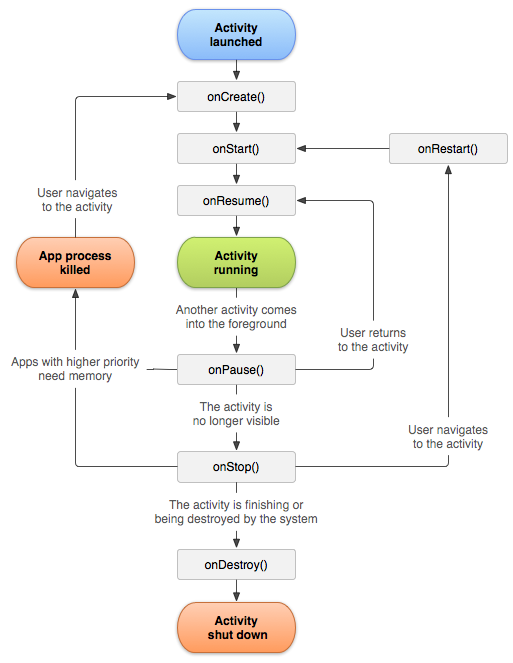
\includegraphics[scale=0.35]{activity_lifecycle.png}
Unterschied Paused/Resume: wird die Activity von einer anderen überdeckt (z.B. Notificationleiste heruntergezogen), wird die erste pausiert (\code{onPause}). Kommt sie wieder in den Vordergrund, wird wieder \code{onResume} aufgerufen.

\code{onPause} ist \textbf{garantiert}. \code{onStop} ist jedoch \textbf{nicht garantiert}. Darum:

\paragraph{Best Practice}

\begin{itemize}
  \item \code{onCreate} erstellt GUI beim Start.
  \item \code{onResume} reagiert auf Benutzereingaben.
  \item \code{onPause} sichert Daten (da die App auch im \code{onStop} oder \code{onDestroy} gekillt werden kann).
  \item \code{onStop} gibt Ressourcen frei.
\end{itemize}

Bei Konfigurationsänderungen wird die Activity neu gestartet. Dazu zählen z.B. \textbf{Screenausrichtungsänderungen}.

Stopped/Started: kommt die Activity wieder in den Vordergrund, weil der User die Applikation nochmal startet oder mit dem Back-Button zurückkommt, wird onRestart aufgerufen.

Destroyed: die App wird vom System destroyed, oder wenn sie explizit vom User geschlossen wird.

\paragraph{Stack}

Activities werden in einem Stack verwaltet, wobei die Activites eines Stacks zu verschiedenen Apps gehören können.\\ 
Eine Gruppe von Activities in einem Stack nennt man auch \textbf{Task}. Es können mehrere Tasks gleichzeitig existieren. Tasks lassen sich im Overview Screen anzeigen.

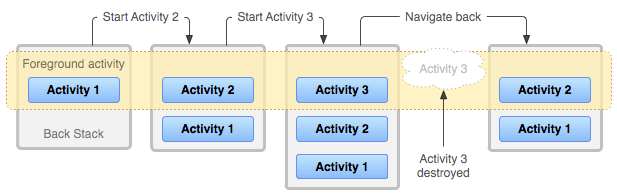
\includegraphics[scale=0.29]{diagram_backstack.png}

\paragraph{Activity Launch Modes} Activities haben verschiedene Launch Modes

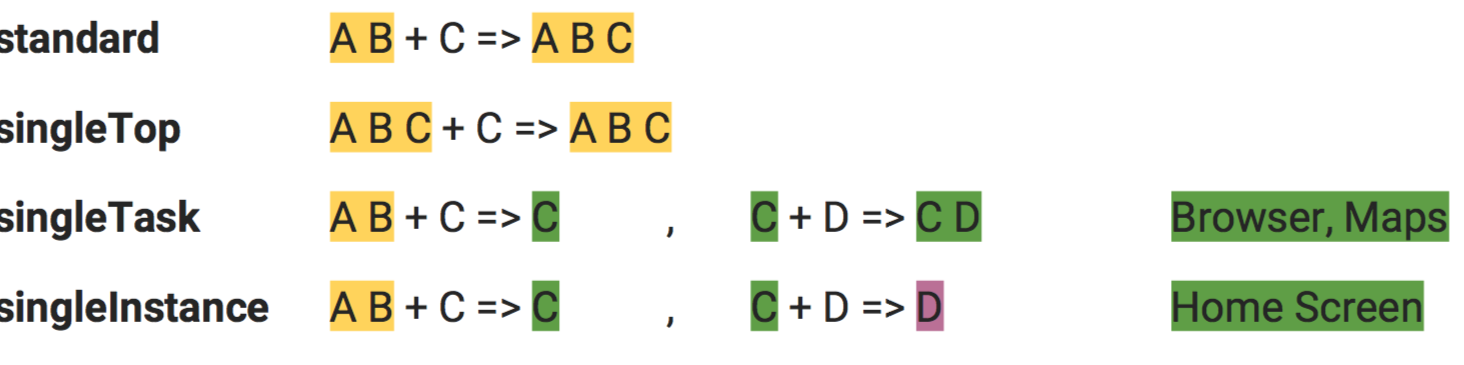
\includegraphics[scale=0.11]{activity-launch-modes.png}

\begin{itemize}
\item \textbf{Standard:} Es wird eine neue Activity in den Stack gepusht
\item \textbf{SingleTop:} Ist Activity A zuoberst auf dem Stack und sie wird nochmals gestartet, wird in Activity A \code{onNewIntent()} ausgeführt
\item \textbf{SingleTask:} Das System erstellt einen neuen Task und instanziert die Activity als die Root des neuen Tasks. Wenn aber schon eine Instanz dieser Activity existiert, wird \code{onNewIntent()} in dieser aufgerufen. 
\item \textbf{SingleInstance:} Es darf nur eine Instanz der Activity geben
\end{itemize}

\paragraph{APK}

Activities (und Ressourcen, etc) werden in ein APK gepackt und installiert. Wird eine Activity aktiv, wird pro APK ein Linux Prozess mit einem Thread gestartet, welcher alle Activities die indiesem APK enthalten sind ausführt. Jedes APK wird unter einem eigenen Linux-User installiert. Inhalt: Libraries, Ressourcen, Assets, Metadaten, kompilierte Klassen im DEX-Format.

Ein APK ist nichts anderes als ein JAR, welches wiederum eine ZIP-Datei ist.

\subsection{Application}
Parent unserer Activities im Manifest ist die Application. Ist auch eine Klasse, die den globalen Zustand unserer App hält. Kann durch eigene Application-Subklasser ersetzt werden. Zugriff aus Activity mit \code{getApplication}, Lifecycle-Methoden: \code{onCreate}, \code{onLowMemory}, \code{onConfigurationChanged}.


\paragraph{Intent} Ein Intent beschreibt was gemacht werden soll und das System entscheidet wer zuständig ist. Apps können selbst wiederum Activites zur Verfügung stellen und bestehende Applikationen ersetzen. Andere Activities können explizit oder implizit aufgerufen werden:
\begin{lstlisting}[language=java]
// Explizit mit Klasse
Intent in = new Intent(this, CalculateActivity.class)
// Implizit mit Aktion
Intent in = new Intent(MediaStore.ACTION_IMAGE_CAPUTRE)
\end{lstlisting}
Andere Activities kann man mit \code{startActivity(intent)} oder \code{startActivityForResult(intent, myId)} starten. Um bei letzterem mit dem Rückgabewert arbeiten zu können muss man \code{onActivityResult} überschreiben.
\begin{lstlisting}[language=java]
@Override
protected void onActivityResult(int request, int result, Intent data) {
  if (result == Activity.RESULT_OK && request == myId) {
    /* ... */
  }
}
\end{lstlisting}
Möchte man einem Intent Daten übergeben, kann man das entweder mit der \code{setData} Methode, welche eine URI entgegennimmt, oder mit \code{putExtra(MediaStore.EXTRA\_OUTPUT, imageCaptureUri)}. Letzere ist eine Struktur mit Key-Value Paaren und nimmt nur primitive Daten, Strings und serialisierbare Datentypen an.

\paragraph{Manifest} Das Manifest enthält Meta-Daten einer App. Es umfasst
\begin{itemize}
\item Komponenten der App
\item Metadaten (Name, Icon, Versionsnummer)
\item Permissions (Internet, kostenpflichtige Anrufe etc.)
\item Anforderungen an die Geräte API
\item \code{minSdkVersion} min-Version des Gerätes
\item \code{targetSdkVersion} höchste Version, mit der getestet wurde
\item Name der Singleton Instanz der Application (Sub-)Klasse.
\end{itemize}

Das Manifest wird vom System verwendet um zu wissen, ob die App installiert werden kann, welche Permissions diese verwendet etc.

\subsection{Android GUI}
\paragraph{Aufbau} Die Basisklasse um User Interfaces zu bauen ist die \code{View}. Eine View ist zuständig seinen Inhalt zu zeichnen und Events zu behandeln. Untergruppen der View sind Widgets und ViewGroups. Widgets ist ein Sammelbegriff für alle fix-fertigen Komponenten für User-Interfaces (Buttons, Images, Checkboxes etc.)
\paragraph{ViewGroup} Die ViewGroup ist eine Unterklasse von View. Sie kann andere View beinhalten. Wenn die ViewGroup beinhaltende View anordnet, spricht man von einem Layout.
\paragraph{Basis Layout} Layouts sind ViewGroups und beschreiben die visuelle Struktur des UIs.
\includegraphics[scale=0.45]{layouts.png}
Die Layout-Parameter beschreiben wie die Views angeordnet und dargestellt werden. Für alle ViewGroups gemeinsam sind \code{android:layout\_width} und \code{android:layout\_height}. Häufig benutze Werte sind \code{match\_parent} (So gross wie mögich, also wie der Parent erlaubt) und \code{wrap\_content} (so klein wie möglich, also wie die Kinder erlauben).\\
In einem \textbf{Linear Layout} werden die Elemente horizontal oder vertikal angeordnet. Mit \code{android:layout\_weight} kann man Elementen ein Gewicht geben, da es selten sinnvoll ist, alle Elemente gleich gross zu lassen. Kinder ohne Weight bekommen minimalen Platz, auf die restlichen wird der verfügbare Platz nach Gewicht aufgeteilt.\\
Das \textbf{Relative Layout} ist das vielseitigse Layout welches Kinder relative zueinander anordnet.
\begin{lstlisting}[language=xml]
<RelativeLayout xmlns:android="... >
  <TextView
    android:text="1. Platz"
    android:id=@+id/first"
    android:layout_centerHorizontal="true" />
  <TextView
    android:text="2. Platz"
    android:id="@+id/first"
    android:layout_below="@id/first"
    android:layout_toStartOf="@id/first" />
  <TextView
    android:text="3. Platz"
    android:id="@+id/textView3"
    android:layout_below="@id/first"
    android:layout_toEnfOf="@id/first" />
</RelativeLayout>
\end{lstlisting}
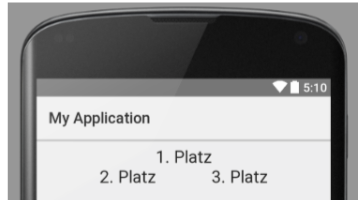
\includegraphics[scale=0.25]{RelativLayout.png} \\
Das \textbf{Frame Layout} kann die Kinder übereinander anordnen (Hilfslinien bei einer Kamera-App).\\
Das Layout muss in der Activity deklariert werden. Dies wird in der Activit Klasse mit \code{setContentView(R.layout.activity\_main)} gemacht.\\

\paragraph{Weitere Layouts}
\begin{itemize}
  \item FlexboxLayout: CSS Flexbox
  \item ConstraintLayout, mit RelativeLayout verwandt (war in Android Studio immer Standard ab irgendeiner Version)
  \item WebView um HTML anzuzeigen: JavaScript kann aktiviert werden, und Java-Objekte können mit JS angesprochen werden
\end{itemize}

\subsection{View finden}
\begin{lstlisting}[language=java]
Button button = (Button) findViewById(R.id.button)
\end{lstlisting}
findViewById innerhalb einer Activity sucht im aktuellen Layout (wahrscheinlich dasjenige von \code{setContentView}). Rückgabe ist immer die Oberklasse \code{View},  das Resultat muss also noch gecastet werden.

Hat man allerdings ein Fragment oder z.B. ein Listenelement, so muss man die Parent-View vorher gespeichert haben (z.B. die Rückgabe des \code{LayoutInflater}), und dann auf dieser die gewünschte View finden. 

\subsection{Widgets}
\paragraph{Button} Vom Button gibt es einen normalen \code{Button} und einen \code{ImageButton} bei dem man mit dem \code{android:src} ein Bild einfügen kann.
\paragraph{Eingabefelder} Der Typ des Eingabefeld bestimmt welche Tastatur verwendet wird. Dies kann man mit dem \code{android:inputType} bestimmen, z.B. \code{textCapSentences}. Es sind auch Kombinationen möglich, z.B. \code{textCapSentences | textAutoCorrect}
\paragraph{Referenzen und ID} Möchte man GUI-Elemente referenzieren, gibt man ihnen einen ID-String, welche Strings sind, die mit \code{@} beginnen. Wenn man einen neue ID definieren will, macht man das mit \code{@+id/}. Das Android-Buildsystem sammelt alle diese IDs als Konstanten in der automatisch generierten Klasse R. Diese Klasse enthält alle Ressourcen als Konstanten. Weitere Resourcesn sind: \code{drawable} (Bilder), \code{menu} (Menüs), \code{mipmap} (Launcher Icon der App) und \code{values} (Strings und andere Konstanten). Mit Aussnahme der values, wird für jeden Ordner eine innere Klasse in R generiert.
\paragraph{Dimensionen in Ressourcen} Konstanten in \code{dimens.xml} werden für Grössen in den Layouts benutzt.
Die Ordnernamen müssen in Java-Namen umgewandelt werden können, dürfen also z.B. kein \code{-} enthalten.

Ressourcen können in mehreren Varianten vorliegen. Die Ordnernamen unterliegen Konventionen, mit denen z.B. Ressourcen-XML für Tablets erstellt werden können, die dann andere Grössenangaben haben.

\begin{lstlisting}[language=xml]
<!-- Layout -->
<RelativeLayout xmlns:android="..." xmlns:tools="..."
  android:layout_width="match_parent"
  android:layout_height="match_parent"
  android:paddingLeft="@dimen/activity_horizontal_margin"
  android:paddingRight="@dimen/activity_horizontal_margin"
  android:paddingTop="@dimen/activity_vertical_margin"
  android:paddingBottom="@dimen/activity_vertical_margin"
  tools:context=".MainActivity">
<!-- dimens.xml -->
  <!-- Default screen margins, per the Android Design guidelines. -->
  <dimen name="activity_horizontal_margin">16dp</dimen>
  <dimen name="activity_vertical_margin">16dp</dimen>
</resources>
\end{lstlisting}
Grössenangeben von Views erfolgen in density-indepentent Pixels (dp oder dip). Bei Schriften verwendet man scale-independent Pixels (sp).
\paragraph{Events und Event Handling}\label{grundlagen:eventhandling} Das Android-Framework hat einen sogenannten Event-Loop (Looper). Dieser wartet bis ein Ereignis passiert und verarbeitet dieses dann. Nur der Main-Thread darf das GUI verändern. \\
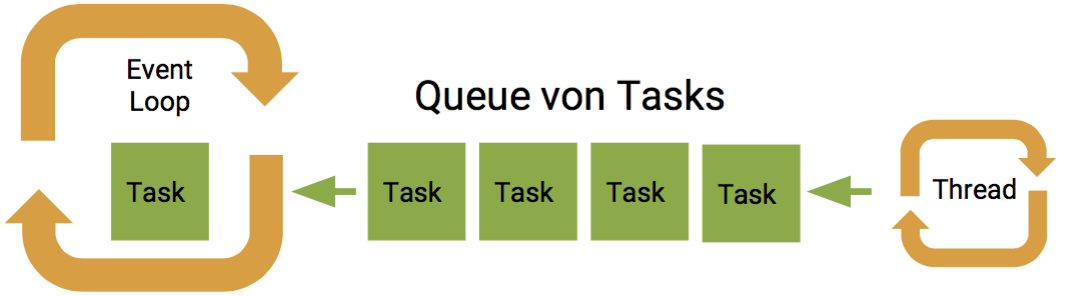
\includegraphics[scale=0.25]{EventLoops.png} \\
Fast alle Listener können mit \code{set[EventName]Listener} registriert werden.
\begin{lstlisting}[language=java]
button.setOnClickListener(new View.OnClickListener() {
  @Override
  public void onClick(View v) {
    /* ... */
  }
});
\end{lstlisting}
Oder onClick Listener in XML deklariert
\begin{lstlisting}[language=xml]
android:onClick="onButtonClicked"
\end{lstlisting}
Alternativ zur anonymen Klasse, kann die Activity auch das Interface implementieren, das kann man mit  (\code{setOnClickListener(this))} bekannt machen.

Ein Listener lässt sich auch bei mehreren Views registrieren. Mit dem übergebenen \code{View}-Parameter kann man unterscheiden (Referenz-Vergleich \code{==}) welches Element den Event ausgelöst hat.

\paragraph{TextWatcher}
Bei der Verarbeitung von Texteingaben haben wir mehrere Möglichkeiten auf Events zu reagieren. Das zu implementierene Interface (\code{TextWatcher}) umfasst 3 Methoden:
\begin{itemize}
\item \code{beforeTextChanged}: Wird aufgerufen bevor der Text geändert wird
\item \code{onTextChanged}: Wird aufgerufen sobald der Text geändert hat
\item \code{afterTextChanged}: Nachdem der Text geändert wurde, kann man den Text noch anpassen (Loop-Gefahr)
\end{itemize}
\begin{lstlisting}[language=java]
editText.addTextChangedListener(new TextWatcher() {
  public void onTextChanged(CharSequence s, int start, int before, int count){ }
  public void beforeTextChanged(CharSequence s, int start, int count, int after){ }
  public void afterTextChanged(Editable s) { }
});
\end{lstlisting}
Bei Eingabefeldern kann man mit \code{setError} Meldungen anzeigen lassen. Dies eignet sich gut für eine Inputvalidierung. Bei jeder Änderung wird diese zurückgesetzt.
\begin{lstlisting}[language=java]
final EditText password = (EditText) findViewById(R.id.password);
password.addTextChangedListener(new TextWatcher() {
  @Override
  public void afterTextChanged(Editable s) {
    String pw = s.toString();
    if (s.length() < 8) {
    password.setError("Passwort muss mindestens 8 Zeichen lang sein.");
    }
  }
  ...
});
\end{lstlisting}
\subsection{Android Testing mit JUnit}
Es gibt mehrere Arten von Tests für eine Activity. Die \code{ActivityUnitTest} manipulieren das UI im Code, die \code{ActivityInstrumentationTestCase2} schickt Clicks und Events an das UI. Um eine App mit mehreren Activities zu testen, gibt es das Espresso Framework, sowie UI Automator um App-übergreifend zu testen.
\begin{lstlisting}[language=java]
public class MainActivityLayoutTest extends ActivityUnitTestCase<MainActivity> {
  public MainActivityLayoutTest() {
    super(MainActivity.class);
  }
  @Override
  protected void setUp() throws Exception {
    super.setUp();
    ContextThemeWrapper context = new
      ContextThemeWrapper(getInstrumentation().getTargetContext(), R.style.AppTheme);
    setActivityContext(context);
    startActivity(
      new Intent(getInstrumentation().getTargetContext(), MainActivity.class),null,null);
}
\end{lstlisting}
Funktionale Tests (ActivityInstrumentationTestCase2) testen eine Activity im echten Systemkontext. Der Test löst Events aus und prüft, ob diese zum erwünschten Resultat führen. Dazu gehören: 
\begin{itemize}
\item Ändert sich das UI wie erwartet
\item Überprüfen von Inputvalidierung
\item Werden Lifecycle Events korrekt behandelt
\end{itemize}
\begin{lstlisting}[language=java]
public class MainActivityInteractionTest extends ActivityInstrumentationTestCase2<MainActivity> {
  public MainActivityInteractionTest() { super(MainActivity.class); }
  public void testSayHi() {
    MainActivity activity = getActivity();
    final EditText editText = (EditText) activity.findViewById(R.id.editText);
    getInstrumentation().runOnMainSync(new Runnable() {
      @Override
      public void run() {
        editText.requestFocus();
      }
    });
    getInstrumentation().waitForIdleSync();
    getInstrumentation().sendStringSync("Hello");
    getInstrumentation().waitForIdleSync();
    Button button = (Button) activity.findViewById(R.id.button);
    TouchUtils.clickView(this, button);
...
\end{lstlisting}

\section{Navigation}
Die Navigation in der App lässt sich durch eine gute Domainanalyse vorbereiten. Mit dieser können die Screens entwickelt werden, die es braucht um mit den Daten umgehen zu können.\\
Danach kann man Screens gruppieren. Dies hilft das Design an grosse und kleine Bildschirme anzupassen (siehe Reflow-Pattern, WED2). Danach kann man die Beziehung zwischen den Screens festlegen. Es gibt die \textbf{Parent-Child} Hierarchie, und die \textbf{Siblings}.
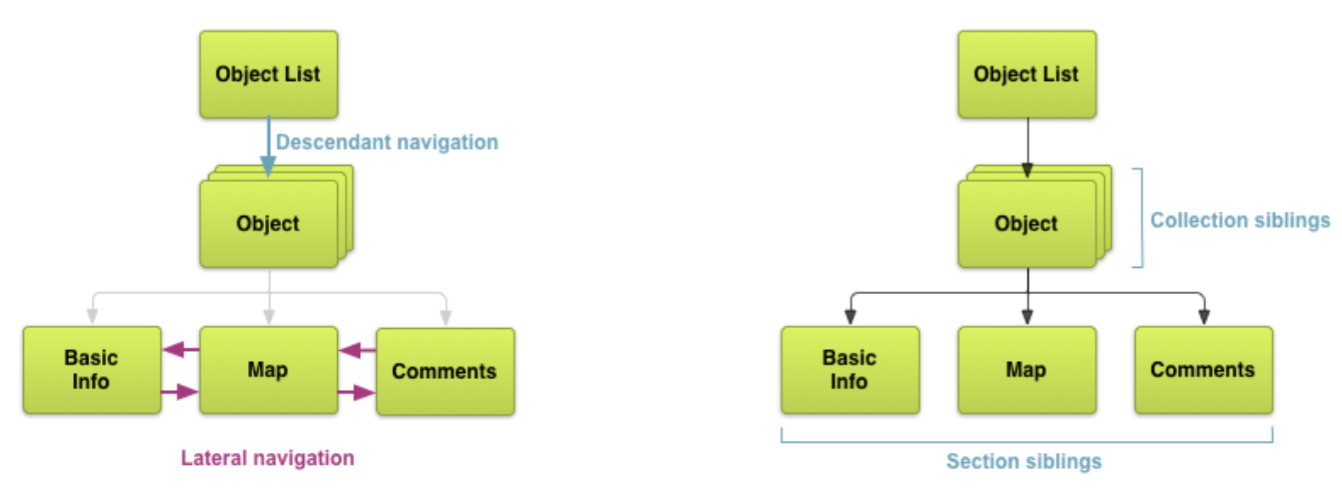
\includegraphics[scale=0.25]{NavScreen.png} \\
Bei der Rückwärtsbeziehung unterscheidet man ebenfalls zwischen 2 Navigationstypen. Die \textbf{Ancestral Navigation} führt zum hierarchischen Parent, die \textbf{Temporal Navigation} führt zum vorherigen Element. Ancestral Navigation geschieht über den Up oder Home Button, Temporal Naviagtion über den Back-Button.\\
Grundsätzlich geht man beim Navigation-Design folgendermassen vor:
\begin{enumerate}
\item Domain-Modell entwerfen
\item Screens ableiten
\item Screens in Beziehung bringen und gruppieren
\item Navigation zwischen den Screens festlegen
\item Wireframe/Storyboard für die Gesamtübersicht erstellen
\item Usability Test mit einem Papier-Prototypen des Wireframes
\end{enumerate}
\paragraph{Fragment} Es ist nicht möglich mehrere Activities auf einem Screen anzuzeigen. Mit Fragments ist das möglich. Ein Fragment ist ein modularer Teil einer Activity mit eigenem Lebenszyklus.
\begin{lstlisting}[language=java]
public class MainActivityFragment extends Fragment {
  public MainActivityFragment() {}
  @Override
  public View onCreateView(LayoutInflater inflater, ViewGroup container, Bundle savedInstanceState) {
  View layout = inflater.inflate(R.layout.fragment_main, container, false);
  counter = (TextView) layout.findViewById(R.id.counter);
  button = layout.findViewById(R.id.button);
  return layout;
  }
}
\end{lstlisting}
Ein Fragment kann im XML in eine Activity eingefügt werden.
\begin{lstlisting}[language=xml]
<?xml version="1.0" encoding="utf-8"?>
<LinearLayout xmlns:android="http://schemas.android.com/apk/res/android"
  android:layout_width="match_parent"
  android:layout_height="match_parent"
  android:orientation="horizontal">
  <fragment xmlns:android="http://schemas.android.com/apk/res/android"
  xmlns:tools="http://schemas.android.com/tools"
  android:id="@+id/fragment"
  android:name="com.example.myfragmentapplication.MainActivityFragment"
  android:layout_width="match_parent"
  android:layout_height="match_parent"
  tools:layout="@layout/fragment_main" />
</LinearLayout>
\end{lstlisting}
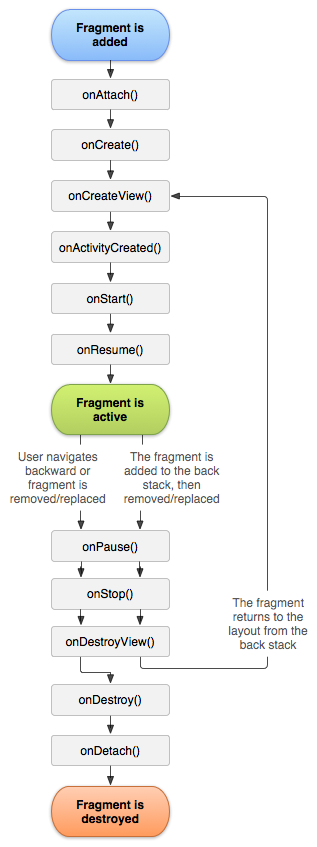
\includegraphics[scale=0.5]{fragment_lifecycle.png}
%TODO: Floating image
Ein Fragment wird einem \code{LayoutInflater} übergeben, der nimmt XML entgegen und instanziert die View Klassen.
Oder dynamisch, mit dem FragmentManager im Java Code
\begin{lstlisting}[language=java]
public class MainActivity extends Activity {
  @Override
  protected void onCreate(Bundle savedInstanceState) {
  super.onCreate(savedInstanceState);
  setContentView(R.layout.activity_main);
  FragmentManager fm = getFragementManager();
  FragmentTransaction ft = fm.beginTransaction();
  MainActivityFragment f = new MainActivityFragment();
  ft.add(R.id.fragment_container, f);
  ft.commit();
  }
...
}
\end{lstlisting}
Best Practice ist, dass Fragments ein Interface zur Kommunikation definieren, welches Parent-Activity implementieren muss.
\begin{lstlisting}[language=java]
public class MainActivityFragment extends Fragement {
  public interface OnItemSelectedlistener {
  void onItemSelected(String item);
  }
  OnItemSelectedListener parentActivity;
  @Override
  public void onAttach(Activity activity) {
  super.onAttach(activity);
  if (!(activity instanceof OnItemSelectedlistener)) throw new AssertionError( "Activity must implement OnItemSelectedlistener!");
  parent = (OnItemSelectedlistener) activity;
  }
}
\end{lstlisting}
\paragraph{Master-Detail Navigation} Die Unterscheidung zwischen den Anzeigevarianten wird über Layouts getroffen. Das Default-Layout der \code{ItemListActivity} beinhaltet nur das \code{ItemListFragment}. Das Tablet enthält ein Linear-Layout mit dem \code{ItemListFragment} sowie ein Platzhalter für das \code{ItemDetailFragment}. Das Kriterium für das Tablet-Layout ist \textit{sw600dp}(smallest width 600dp).
\begin{lstlisting}[language=java]
public clas ItemListActivity extends Activity implements ItemListFragment.Callbacks {
  private boolean twoPane;
  @Override
  protected void onCreate(Bundle savedInstanceState) {
  super.onCreate(savedInstanceState);
  setContentView(R.layout.activity_item_list);
  if(findViewById(R.id.item_details_container) != null) {
    twoPane = true;
  }
  }
  @Override
  public void onItemSelected(String id) {
  if(twoPane) {
    Bundle arguments = new Bundle();
    arguments.putString(ItemDetailFragment.ARG_ITEM_ID, id);
    ItemDetailFragment fragment = new ItemDetailFragment();
    fragment.setArguments(arguments);
    getFragmentManager()
    .beginTransaction()
    .replace(R.di.item_detail_container, fragment)
    .commit();
  } else {
    Intent detailIntent = new Intent(this, ItemDetailActivity.class);
    detailIntent.putExtra(ItemDetailFragment.ARG_ITEM_ID, id);
    startActivity(detailIntent);
  }
  }
}
\end{lstlisting}
Activities sollte man verwenden, wenn man einen Einstiegspunkt in einen Task braucht. \textbf{Wichtig:} Activities leben weiter, wenn wir eine neue Activity starten.

Neben \code{fragmentTransation.add} gibt es noch \code{fragmentTransaction.replace}. Es kann auch direkt \code{replace} aufgerufen werden, auch wenn noch keines ge-addet wurde. Beispiel siehe Spick ''Settings Page''.

\subsection{Activity-Layout für dynamisch}
Frame Layout ''hat sich so eingebürgert''.
\begin{lstlisting}[language=xml]
<LinearLayout>
  <FrameLayout android:id="@+id/fragment_container"/>
</LinearLayout>
\end{lstlisting}

\paragraph{Callback}
Damit Fragments mit der Activity kommunizieren können:
\begin{enumerate}
  \item Interface definieren. Am besten ''event-mässig'', also \code{onEVENT}
  \item Interface auf Activity implementieren
  \item in Fragment im \code{onAttach}:\\ \code{if !(activity instanceof INTERFACE) throw new AssertionError}
\end{enumerate}

\subsection{Verschachtelung}
Ab Android 4.2, API-Level 17, können Fragments verschachtelt werden. Dann muss man mit dem \code{getChildFragmentManager} gearbeitet werden, z.B. beim ViewPager.

\subsection{Backbutton}
\begin{lstlisting}[language=java]
// vorher/nachher:
.replace().commit();
.replace().addToBackStack(null).commit();

public void onBackPressed()  {
  if (getFragmentManager().getBackStackEntryCount() <= 1) { 
  finish();
  } else {
  pages.pop();
  getFragmentManager().popBackStack();
  }
}
\end{lstlisting}

\subsection{Menus}
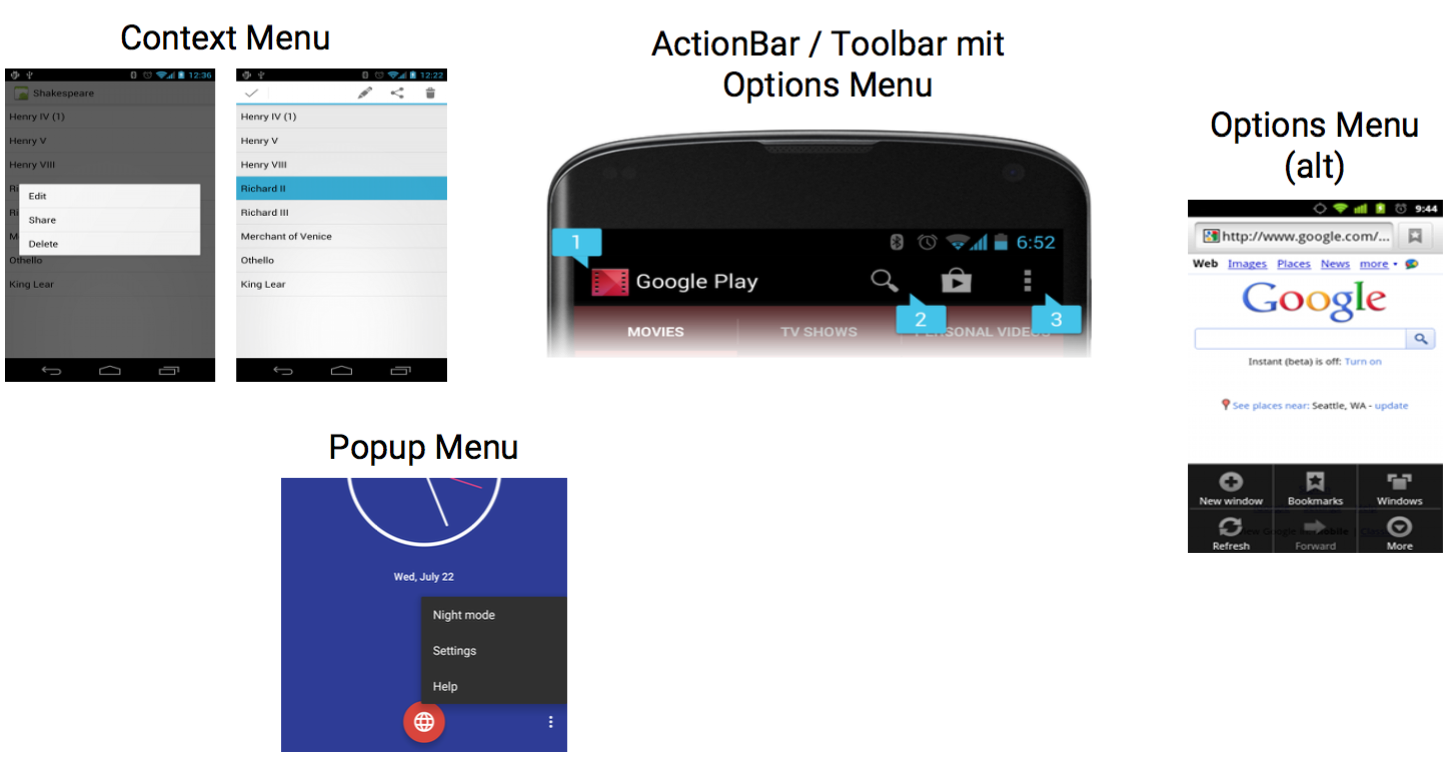
\includegraphics[scale=0.25]{Menus.png}
\paragraph{Options Menu} Das Options Menu ist teil der ActionBar. Es enthält Actions die generell für die App/Activity gedacht sind. Apps mit Navigation Drawer haben teilweise kein Options Menu mehr. \\
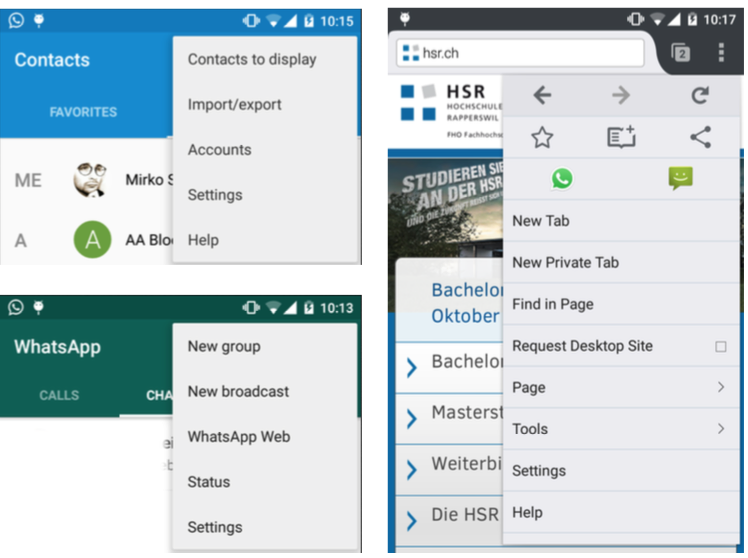
\includegraphics[scale=0.25]{OptionsMenu.png}
\begin{lstlisting}[language=java]
public boolean onCreateOptionsMenu(Menu menu) {
  menu.add(0, START_MENU_ITEM, 0, "Start");
  menu.add(0, SUBMIT_MENU_ITEM, 0, "Submit");
  return true;
}
public boolean onOptionsItemSelected(MenuItem item){
  switch(item.getItemId()){
  case START_MENU_ITEM:
    // start
    return true;
  case SUBMIT_MENU_ITEM:
    // submit
    return true;
  }
  return super.onOptionsItemSelected(item);
}
\end{lstlisting}
Der bessere Ansatz wäre die deklarative Implementation im XML.
\begin{lstlisting}[language=xml]
<menu xmlns:android="http://schemas.android.com/apk/res/android"
xmlns:tools="http://schemas.android.com/tools" tools:context=".MainActivity">
  <item android:id="@+id/action_search"
  android:title="@string/action_search"
  android:icon="@drawable/ic_action_search"
  android:orderInCategory="100"
  android:showAsAction="never" />
  <item android:id="@+id/action_settings"
  android:title="@string/action_settings"
  android:orderInCategory="100"
  android:showAsAction="never" />
</menu>
\end{lstlisting}
\begin{lstlisting}[language=java]
public class MainActivity extends Activity {
  public boolean onCreateOptionsMenu(Menu menu) {
  getMenuInflater().inflate(R.menu.menu_main, menu);
  return true;
  }
  public boolean onOptionsItemSelected(MenuItem item) {
  /* ... */
  }
}
\end{lstlisting}
\paragraph{Settings-Page} Die Settings-Page erbt von der Klasse \code{PreferenceActivity}. Sie kann im \code{PreferenceScreen} Tag definiert werden.
\begin{lstlisting}[language=xml]
<!-- preferences.xml -->
<PreferenceScreen xmlns:android="...">
  <CheckBoxPreference
  android:defaultValue="true"
  android:key="@string/sync_pref"
  android:title="Synchronize" />
  <MultiSelectListPreference
  android:entries="@array/languages"
  android:entryValues="@array/languages"
  android:key="@string/lang_pref"
  android:title="Languages" />
</PreferenceScreen>
<!-- resources.xml -->
<resources>
  <string name="lang_pref">language</string>
  <string name="sync_pref">synchronize</string>
  <string-array name="languages">
  <item>German (CH)</item>
  <item>English (UK)</item>
  </string-array>
</resources>
\end{lstlisting}
\begin{lstlisting}[language=java]
public class Preferences extends PreferenceActivity {
  @Override
  public void onCreate(Bundle savedInstanceState) {
  super.onCreate(savedInstanceState);
  getFragmentManager()
    .beginTransaction()
    .replace(R.id.content, new PrefsFragment()
    .commit();
  PreferenceManager.setDefaultValues(this, R.xml.preferences, false);
  }
  public static class PrefsFragment extends PreferenceFragment {
  @Override
  public void onCreate(Bundle savedinstanceState) {
    super.onCreate(savedInstanceState);
    addPreferencesFromResource(R.xml.preferences);
  }
  }
}
\end{lstlisting}
In der MainActivity mit dem Settings-Menueintrag brauchen wir bloss noch die neue Activity zu starten.
\begin{lstlisting}[language=java]
@Override
public boolean onOptionsItemSelected(MenuItem item){
  int id = item.getItemId();
  if(id == R.id.action_settings) {
  startActivity(new Intent(this, Prefernces.class));
  return true;
  }
  return super.onOptionSItemSelected(item);
}
\end{lstlisting}
Die Einstellung wird mittels dieser Funktion ausgelesen.
\begin{lstlisting}[language=java]
SharedPreferences settings = getSharedPreferences(FILENAME, 
  MODE_PRIVATE); // alternativ: MODE_MULTI_PROCESS
SharedPreferences.Editor editor = settings.edit();
editor.putBoolean("disabled", false)

boolean isDisabled = settings.getBoolean("disabled", false)
// false ist Defaultwert falls nicht existent

editor.commit();
\end{lstlisting}
Auch Fragments können Einträge dem Menu der Activity hinzufügen. Die Behandlung erfolgt analog entweder im Fragment oder in der Activity.
\begin{lstlisting}[language=java]
public class MainFragment extends Fragment {
  @Override
  public void onCreateOptionsMenu(Menu menu, MenuInflater inflater) {
  inflater.inflate(R.menu.menu_main, menu);
  }
  @Override
  public void onCreate(Bundle savedInstanceState) {
  super.onCreate(savedInstanceState);
  setHasOptionsMenu(true);
  }
}
\end{lstlisting}
\paragraph{Context und Popup Menu} Ein Context Menü für Actions welche die selektierte View betreffen. Meist ändert sich bei einer Selektion die ActionBar.\\
Popup Menüs lassen sich z.B an einen beliebigen Button binden (Vergleichbar mit einem Spinner/Combobox). \\
Popup Menus eignen sich für Overflow-Style Menu für Actions die Context spezifisch sind (beispielsweise Weiterleiten und Antworten bei Mail). 
\begin{lstlisting}[language=xml]
<ImageButton
  android:layout_width="wrap_content" 
  android:layout_height="wrap_content" 
  android:src="@drawable/ic_overflow_holo_dark"
  android:contentDescription="@string/descr_overflow_button"
  android:onClick="showPopup" />
\end{lstlisting}
\begin{lstlisting}[language=java]
public void showPopup(View v) {
  PopupMenu popup = new PopupMenu(this, v);
  MenuInflater inflater = popup.getMenuInflater();
  inflater.inflate(R.menu.actions, popup.getMenu());
  popup.show();
}
\end{lstlisting}
\paragraph{Action Bar} Die ActionBar war der erste Versuch eine normierte "{}Schnittstelle"{} für Aktionen in einer App zu kreieren. \\
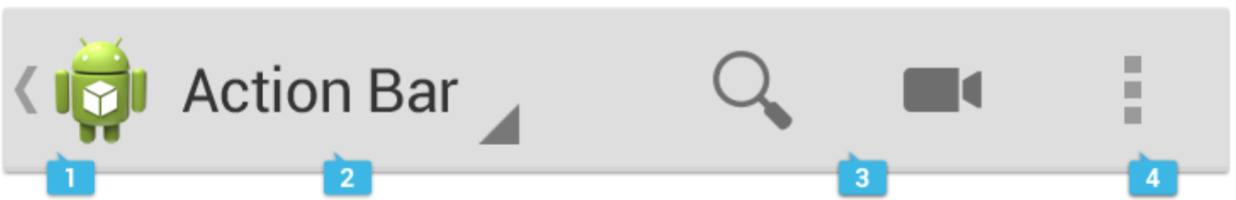
\includegraphics[scale=0.25]{ActionBar.png}
\begin{enumerate}
\item App Icon und ev. Up-/Home-Navigation
\item Name der App oder View-Switcher
\item Actions (Teil des Options Menu)
\item Action-Overflow mit dem Rest des Menus
\end{enumerate}
\paragraph{Toolbar} Die Toolbar soll ab Android 5.0 die ActionBar ablösen. Sie ist flexibler aber noch nicht so weit verbreitet. Um sie in älteren Android Versionen verwenden zu können ist eine Support-Library nötig.

\includegraphics[scale=0.35]{toolbar.png}
\begin{lstlisting}[language=xml]
<RelativeLayout xmlns:android="..." xmlns:app="..." xmlns:tools="..."
  android:layout_width="match_parent" android:layout_height="match_parent"
  tools:context=".MainActivity">
  <android.support.v7.widget.Toolbar
  android:id="@+id/toolbar"
  android:layout_width="match_parent"
  android:layout_height="wrap_content">
  </android.support.v7.widget.Toolbar>
  <fragment
  ...
  android:layout_below="@+id/toolbar"
  tools:layout="@layout/fragment_main" />
</RelativeLayout>
\end{lstlisting}
Damit die Toolbar als ActionBar funktioniert braucht es zusätzliche Konfiguration im Java Code
\begin{lstlisting}[language=java]
public class MainActivity extends AppCompatActivity {
  @Override
  protected void onCreate(Bundle savedInstanceState) {
  super.onCreate(savedInstanceState);
  setContentView(R.layout.activity_main);
  Toolbar toolbar = (Toolbar)findViewById(R.id.toolbar);
  setSupportActionBar(toolbar);
  }
}
\end{lstlisting}
\paragraph{Navigation Drawer} Dies ist eine Art Hauptmenü. Es wechselt zwischen Activities oder Fragments. Es können auch gewisse Einstellungen verändert werden (Toggle). \\
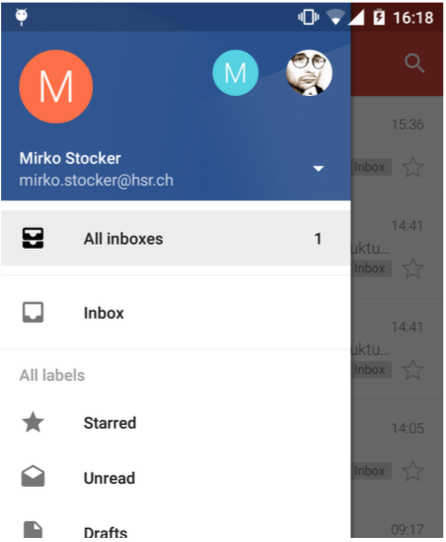
\includegraphics[scale=0.35]{navigationdrawer.png} \\
Der Drawer benötigt eine Layoutdefinition und eine Menudeklaration. Das Layout der Activity ist rechts vom Navigation Drawer und braucht ein FrameLayout.
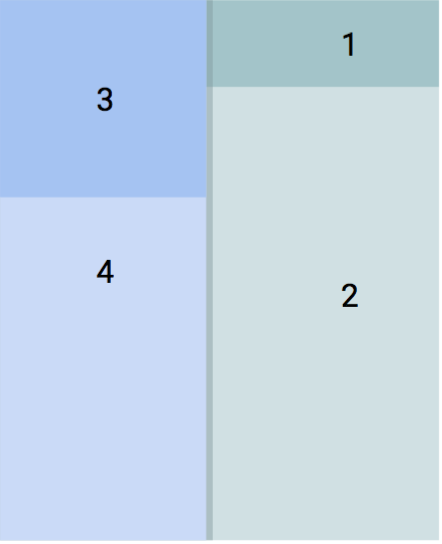
\includegraphics[scale=0.25]{NavDrawer.png}
1. Toolbar, 2. Content, 3. Header, 4. Menu-Items
\begin{lstlisting}[language=xml]
<android.support.v4.widget.DrawerLayout xmlns:android="..." xmlns:app="..." xmlns:tools="..."
  android:id="@+id/drawer_layout"
  android:fitsSystemWindows="true"
  tools:context=".MainActivity">
  <FrameLayout
  android:id="@+id/content"
  android:orientation="vertical">
  <android.support.v7.widget.Toolbar
    android:id="@+id/toolbar"/>
  <TextView ... />
  </FrameLayout>
  <android.support.design.widget.NavigationView
  android:id="@+id/navigation_view"
  android:layout_gravity="start"
  app:headerLayout="@layout/drawer_header"
  app:menu="@menu/drawer" />
</android.support.v4.widget.DrawerLayout>
\end{lstlisting}
In der Activity kann ein Listener registriert werden, welcher auf Menüpunkte des Drawers reagiert.
\begin{lstlisting}[language=java]
NavigationView view = (NavigationView)findViewById(R.id.navigation_view);
view.setNavigationItemSelectedListener(
  new NavigationView.OnNavigationItemSelectedListener() {
  @Override
  public boolean onNavigationItemSelected(MenuItem item) {
  item.setChecked(true);
  drawerLayout.closeDrawers();
  return true;
  }
});
\end{lstlisting}

\paragraph{Menüs}
Im Handler: \code{true} bedeutet ''behandelt''.

Von Fragments aus können auch Menü-Optionen hinzugefügt werden. Dazu gibt es auch dort \code{onCreateOptionsMenu(Menu menu, MenuInflater inflater)}, dort wird der Inflater also bereits mitgegeben.

In \code{onCreate} muss unbedingt \code{setHasOptionsMenusetHasOptionsMenu(true)} gesetzt werden, sonst wird wahrscheinlich das Callback nie aufgerufen
\paragraph{Toast und Snackbar} Toast sind kleine Feedbacknachrichten. Sie werden mit \code{Toast.makeText(...).show()} angezeigt.
\section{Design Patterns}
\subsection{Listen}
Listen sind ein häufig verwendets UI-ELement. \code{ListView} und \code{ExpandableListView} sind die implementierenden Klassen. Die Einträge können komplexe Layouts sein und es könne beliebige Java-Objekte dargestellt werden.
\begin{lstlisting}[language=xml]
<ListView
  android:layout_width="match_parent"
  android:layout_height="match_parent"
  android:id="@+id/listView"/>
\end{lstlisting}
Da die ListView mit allen Java Klassen umgehen können muss, verwendet es das Adapter Design Pattern. Das Datenmodell soll unabhängig von der ListView bleiben, und der Adapter vermittelt zwischen Daten-Klassen und ListView.\\
ListView und GridViews sind AdapterViews. Für das zuweisen eines Adapters wird \code{setAdapter()} verwendet.
\begin{lstlisting}[language=xml]
ArrayAdapter<String> adapter = new ArrayAdapter<>(this, R.layout.rowlayout, R.id.label);
listView.setAdapter(adapter);
\end{lstlisting}
Möchte man einen eigenen ArrayAdapter implementieren muss man in diesem die \code{getView} Methode überschreiben um zu kontrollieren, wie genau ein Eintrag aussieht.
\begin{lstlisting}[language=java]
View getView(int position, View convertView, ViewGroup parent);
\end{lstlisting}
Wobei \code{position} der Index ist, der dargestellt werden soll, \code{convertView} die alte View (oder null) ist, und \code{parent} den zukünftigen Parent. Die alte View wird aus Performancegründen mitgegeben, damit nicht immer eine neue Instanz des Layouts erstellt sondern nur die Daten aktualisiert werden. Eine ListView mit Checkboxen:
\begin{lstlisting}[language=java]
public View getView(int position, View convertView, ViewGroup parent) {
  final Module module = moduleList.get(position);
  if(convertView == null) {
  LayoutInflater lf = (...)getSystemService(Context.LAYOUT_INFLATER_SERVICE);
  convertView = lf.inflate(R.layout.rowlayout, null);
  }
  TextView tv = (...)convertView.findViewById(R.di.textView);
  CheckBox cb = (...)convertView.findViewById(R.id.checkbox);
  tv.setText("(" + module.getCode() + ")");
  cb.setText(module.getName());
  cb.setChecked(module.isSelected());
  cb.setOnClickListener(new View.OnClickListener() {
  @Override
  public void onClick(View v) {
    CheckBox b = (...)v;
    module.setSelected(!b.isChecked());
  }
  });
  return convertView;
}
\end{lstlisting}
Die Performance der ListView ist nur bedingt gut. \code{findViewById} sind teure Operationen und diese werden mit komplexeren Layouts mehr. 
\paragraph{View Tags} Views können getagged werden (\code{setTag(Object tag)}). Man kann das mit einem Key-Value Paar machen oder einfach mit einem Object. So kann man beliebige Daten an eine View anhängen. 
\subsection{Recycler View} 
Die RecylcerView hat mehrere Verbesserungen gegenüber den anderen beiden Views. Es können mehrere Layoutmanager definiert werden, es können Animationen für Hinzufügen und Entfernen von Einträgen gesetzt werden, und das Recyling von Elementen wurde fest eingebaut. Leider ist es mit der RecyclerView mühsamer das Click-Handling zu implementieren. Die Komponenten der RecylcerView sind:
\begin{itemize}
\item \textbf{Adapter:} Analog zu eigenem ArrayAdapter (leicht anderes API)
\item \textbf{ViewHolder:} Klasse welche die Views zwischenspeichert
\item \textbf{LayoutManager:} Defaults für übliche Layouts (optional)
\item \textbf{ItemDecorator:} Trennlinien oder andere Dekoratoren um die Elemente (optional)
\item \textbf{ItemAnimator:} Animiert hinzufügen, entfernen und scrolling von Elementen (optional)
\end{itemize}
\begin{lstlisting}[language=java][caption="RecyclerView Schnittstelle"]
public class MyAdapter extends RecyclerView.Adapter<ViewHolder> {
  private ArrayList<Module> dataset;
  public MyAdapter (ArrayList<Module> modules) {dataset = modules;}
  public ViewHolder onCreateViewHolder(ViewGroup parent, int viewType){ 
  /* --- */
  }
  public onBindViewHolder(ViewHolder holder, int position) {
  /* ... */
  }
}
\end{lstlisting}

\subsection{RecyclerView}
Statt einer \code{ListView} nimmt man einfach eine \code{RecyclerView} (XML). Der Adapter ist dann aber anders als ein \code{ListView}-Adapter. Folgend ein \code{RecyclerView.Adapter}
\begin{lstlisting}[language=java]
public class NotesAdapter extends 
  RecyclerView.Adapter<NotesAdapter.ViewHolder> {
private Notes data;
private ItemSelectionListener selectionListener;

public NotesAdapter(Notes notes, 
  ItemSelectionListener selectionListener) {
  this.data = notes;
  this.selectionListener = selectionListener;
}
class ViewHolder extends RecyclerView.ViewHolder {
  TextView textView;
  ViewHolder(View itemRoot) {
    super(itemRoot);
    textView = itemRoot.findViewById(R.id.textView);
    textView.setOnClickListener(new View.OnClickListener() {
      @Override
      public void onClick(View view) {
        selectionListener.onItemSelected(
          ViewHolder.this.getAdapterPosition());
      }
    });
  }
}
@Override
public ViewHolder onCreateViewHolder(ViewGroup parent, 
  int viewType) {
  LayoutInflater inflater = LayoutInflater.from(parent.getContext());
  View view = inflater.inflate(R.layout.rowlayout, parent, false);
  return new ViewHolder(view);
}
@Override
public void onBindViewHolder(final ViewHolder holder, 
  final int position) {
  holder.textView.setText(data.get(position).getTitle());
}
@Override
public int getItemCount() {
  return data.getSize();
}
}
\end{lstlisting}

Die RecyclerView bemerkt Änderungen an den Daten nicht von selbst. Um eine Aktualisierung zu veranlassen:
\begin{itemize}
  \item \code{notifyDataSetChanged()}
  \item \code{notifyItemChanged(positionToUpdate)}
  \item \code{notifyItemInserted(insertPosition)}
  \item \code{notifyItemRemoved(removePosition)}
\end{itemize}

Diese gibts auch noch in einer \code{notifyItemRange}-Variante
\subsection{Design und Architektur Patterns}
Um viele Klassen zu ordnen kann man beispielsweise die Multitier Architecture verwenden. Darin sind die Abhängigkeiten klar gerichtet und es existieren keine Zyklen. Um nun die Domain überwachbar zu machen, kann man das Observer Pattern implementieren.
\paragraph{Swipe Refresh} Anstelle, dass unsere App sich selbst aktualisiert kann man das mit einem Swipe Refresh machen. Dafür braucht man eine Support Library.
\begin{lstlisting}[language=xml]
<android.support.v4.widget.SwipeRefreshLayout>
  <android.support.v7.widget.RecyclerView/>
</android.support.v4.widget.SwipeRefreshLayout>
\end{lstlisting}
\begin{lstlisting}[language=java]
final SwipeRefreshLayout swipe = 
  (SwipeRefreshLayout) findViewById(R.id.swipeRefreshLayout);
swipe.setOnRefreshListener(new SwipeRefreshLayout.OnRefreshListener() {
  public void onRefresh() {
  /*...*/
  swipe.setRefreshing(false);
  }
});
\end{lstlisting}

\section{Material Design}
Material Design ist eine Design Sprache (Design Language). Eine Design Sprache ist eine Hilfestellung für den Designprozess. Es beschreibt, wie die Teile einer Applikation aussehen und sich verhalten sollen. Material ist die Metapher und arbeitet im 3D-Raum mit Licht und Schatten. Es ist angelehnt an physikalische Begebenheiten. Man verwendet ein Grid für die Ausrichtung und versucht, wenn angemessen eine Reaktion auf User-Input zu geben. Materials sind geometrische Formen (Schnipsel aus Papier) mit einer Dicke von exakt 1dp. Duch die unterschiedliche Anordnung auf der Z-Achse entsteht Schatten. Dieses Konzept hat Einfluss auf verschiedene Aspekte. Material Design Styleguides umfasset deshalb auch: Layout, Style, Animation, Components, Patterns und Usability.\\
\paragraph{Layout} Grundelement ist das Papier, das an- und übereinander gelegt werden kann. Ein Floating Action Button beispielsweise, bietet eine Aktionsmöglichkeit für das Papier. Alle anderen Materialien werden an einem 8dp Grid ausgerichtet.
\paragraph{Layout Spacing} Der Abstand zwischen Elementen ist meist ein Vielfaches von 8. \\
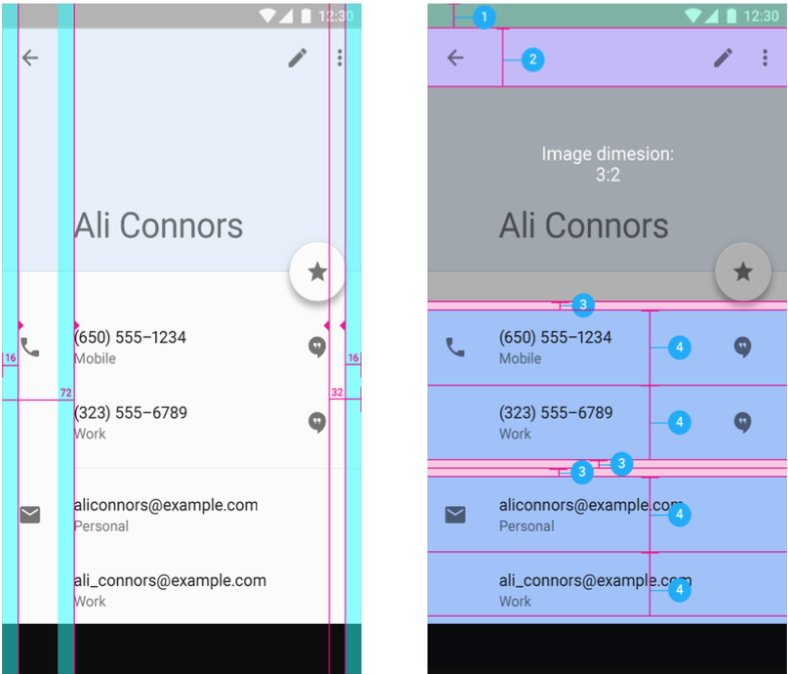
\includegraphics[scale=0.25]{LayoutSpacing.png}
\begin{enumerate}
\item Status bar: 24dp
\item Toolbar: 56dp
\item Space: 8dp
\item List item: 72dp
\end{enumerate}
\paragraph{Style} Für Material Design wird empfohlen, dass man 3 Farbtöne der Primärpalette und eine Akzentfarbe aus einer zweiten Palette wählt. 
\paragraph{Animation} helfen die Illusion aufrecht zu halten, dass wir die Materialien auf dem Screen direkt manipulieren (wie durch eine Glasscheibe). Man sollte visuelles Feedback auf Input geben und den Übergang zwischen Zuständen animieren. 
\paragraph{Usability} Wichtige Punkte in Usability sind:
\begin{itemize}
\item Touch-Targes nicht zu klein machen
\item Navigation soll nachvollziehbar und nicht komplex sein
\item Fontgrössen, Farben
\item RTL-Layouts werden (wenn richtig gemacht automatisch) gespiegelt
\item Texte in Grafiken sind problematisch
\end{itemize}
\subsection{Umsetzung}
\paragraph{View Styling} Views können direkt im XML-Layout gestyled werden. 
\begin{lstlisting}[language=xml]
<Button
  android:layout_width="wrap_content"
  android:layout_height="wrap_content"
  android:text="New Button"
  android:id="@+id/button2"
  android:layout_gravity="center"
  android:background="#ff85e1"
  android:height="36dp"
  android:minWidth="64dp"
  android:padding="8dp" />
\end{lstlisting}
Meist ist es am schönsten wenn man so etwas in ein Style auslagert.
\begin{lstlisting}[language=xml]
<style name="MyButtonStyle">
  <item name="android:background">#ff85e1</item>
  <item name="android:height">36dp</item>
  <item name="android:minWidth">64dp</item>
  <item name="android:padding">8dp</item>
</style>
\end{lstlisting}
Dies wird dann mit \code{style="@style/MyButtonStyle"} referenziert. Auch diese Ressourcen können für unterschiedliche Geräte, Versionen etc. spezifiziert werden. 
\paragraph{Themes} sind Styledefinitionen die für eine Activity oder App gelten
\begin{lstlisting}[language=xml]
<application
  ...
  android:theme="@style/AppTheme">
  <activity
  android:name".MainActivity"
  android:theme="@style/AppTheme" >
\end{lstlisting}
Das AppTheme ist das Standarttheme, und müsste nicht spezifiziert werden. Im \code{styles.xml} kann man die entsprechenden Styles definieren.
\begin{lstlisting}[language=xml]
<style name="AppTheme" parents="Theme.AppCompat.Light.NoActionBar">
<!-- Ueberschreiben von Theme einstellungen -->
</style>
\end{lstlisting}
Im Theme definierte Styles können in anderen Ressourcen referenziert werden, anstelle eines \@ wird ein ? verwendet. Bei der Syntax gibt es zwei Varianten:
\begin{lstlisting}[language=xml]
<!-- colorAccent ist im Theme definiert -->
<style name="AccentedButton">
  item name="android:background">?colorAccent
</style>
<Button android:background="?attr/colorAccent" />
<!-- gleich wie -->
<Button android:background="?/colorAccent" />
\end{lstlisting}


Die Aktzenfraben können im Style.xml definiert werden
\begin{lstlisting}[language=xml]
<item name="primary" type="color">#3F51B5</item>
<item name="primary_dark" type="color">#303F9F</item>
<item name="accent" type="color">#FF4081</item>
\end{lstlisting}
\paragraph{Theme Overlays} Die Kombination von Light-Theme und dunkler Toolbar führt dazu, dass die Schrift in der Toolbar schwarz ist. View können keine eigenen Themes haben, aber Theme Overlays, die einen Teil der Theme-Attribute überschreiben.
\begin{lstlisting}[language=xml]
<android.support.v7.widget.Toolbar
  ...
  app:theme="@style/ThemeOverlay.AppCompat.Dark.ActionBar"
  app.popupTheme="@style/ThemeOverlay.AppCompat.Light" />
\end{lstlisting}
\paragraph{Floating Action Button} Der FAB bietet eine primäre Aktion für die darunterliegende View an.
\begin{lstlisting}[language=xml]
<android.support.design.widget.FloatingActionButton
  android:src="@drawable/plus"
  android:onClick="onPlusClicked" />
\end{lstlisting}
\paragraph{TextInputLayout} Dies ist ein EditText, bei dem der Hinweistext beim editieren nicht verschwindet.
\begin{lstlisting}[language=xml]
<android.support.design.widget.TextInputLayout
  android:id="@+id/username_text_input_layout"
  android:layout_width="match_parent"
  android:layout_height="wrap_content
  android:layout_gravity="center" >
  <EditText
  android:id="@+id/username_edit_text"
  android:layout_width="match_parent"
  android:layout_height="wrap_content"
  android:hint="Your username"
  android:layout_gravity="center" />
</android.support.design.widget.TextInputLayout>
\end{lstlisting}
\paragraph{Scrollende Toolbar} Die Toolbar kann auch mit dem Inhalt weggescrollt werden. 
\begin{lstlisting}[language=xml]
<android.support.design.widget.CoordinatorLayout xmlns:android="..." xmlns:app="..."
  android:layout_width="match_parent" android:layout_height="match_parent">
  <android.support.v7.widget.RecyclerView
  android:id="@+id/recyclerView"
  android:layout_width="match_parent"
  android:layout_height="match_parent"
  app:layout_behavior="@string/appbar_scrolling_view_behavior" />
  <android.support.design.widget.AppBarLayout
  android:id="@+id/appBarLayout"
  android:layout_width="match_parent"
  android:layout_height="wrap_content">
  <android.support.v7.widget.Toolbar
  android:id="@+id/toolbar"
  android:layout_width="match_parent"
  android:layout_height="?attr/actionBarSize"
  app:layout_scrollFlags="scroll|enterAlways"/>
</..>
\end{lstlisting}
\paragraph{Zusammenklappbare Toolbars} Toolbars die Verschwinden können.
\begin{lstlisting}[language=java]
<android.support.design.widget.AppBarLayout
  ...
  android:layout_height="128dp">
  <android.support.design.widget.CollapsingToolbarLayout
  android:id="@+id/collapsing_toolbar"
  android:layout_width="match_parent"
  android:layout_height="match_parent"
  app:contentScrim="?attr/colorPrimary"
  app:expandedTitleMarginEnd="64dp"
  app:expandedTitleMarginStart="48dp"
  app:layout_scrollFlags="scroll|exitUntilCollapsed">
  <android.support.v7.widget.Toolbar
  android:id="@+id/toolbar"
  android:layout_width="match_parent"
  android:layout_height="?attr/actionBarSize"
  app:layout_collapseMode="pin" />
\end{lstlisting}
\paragraph{Tab Navigation} Dies ist kein neues Feature, aber mit dem CoordinatorLayout und AppBarLayout integriert worden. Tabs sind unterschiedliche Screens (Fragments), und Swipe oder Touch wechselt zwischen Tabs.
\begin{lstlisting}[language=xml]
<CoordinatorLayout>
  <AppBarLayout>
  <Toolbar />
  <TabLayout />
  </AppBarLayout>
  <ViewPager />
</CoordinatorLayout>
\end{lstlisting}
Das TabLayout zeigt die Liste der Tabs an, der ViewPager den Inhalt der Tabs (wechselt zwischen Fragments).
\begin{lstlisting}[language=java]
@Override
protected void onCreate(Bundle savedInstanceState) {
  ...
  ViewPager vp = (...)findViewById(R.di.viewpager);
  ViewPagerAdapger adapter = new ViewPagerAdapger(getSupportFragmentManager());
  adapter.addFragment(new ListFragment(), "CALLS");
  adapter.addFragment(new ListFragment(), "CHATS");
  adapter.addFragment(new ListFragment(); "CONTACTS");
  vp.setAdapter(adapter);
  TabLayout tl = (...)findViewById(R.id.tabs);
  tl.setupWithViewPager(vp);
\end{lstlisting}
Diese Toolbar lässt sich beim Scrollen auch verstecken.
\begin{lstlisting}[language=java]
<android.support.design.widget.CoordinatorLayout ...>
  <android.support.design.widget.AppBarLayout ...>
  <android.support.v7.widget.Toolbar ...
    app:layout_scrollFlags="scroll|enterAlways />
  <android.support.design.widget.TabLayout .../>
  </android.support.design.widget.AppBarLayout>
  <android.support.v4.view.ViewPager ..
  app:layout_behavior="@string/appbar_scrolling_view_behavior" />
</android.support.design.widget.CoordinatorLayout>
\end{lstlisting}
Dies klappt jedoch nur, wenn die Fragments RecylcerView oder NestedScrollViews sind (nicht mit ListViews oder ScrollViews).
\section{Persistenz}
Die Apps werden vom System beendet, ohne dass dies dem Benutzer bewusst ist. Das Sichern der Daten ist also Aufgabe der App. Es gibt zwei unterschiedliche Arten von Daten: Zustandsdaten der Views und Anwendungsdaten der Domain-Klassen.
\paragraph{View-Daten Persistieren} \code{onCreate} und \code{onSaveInstanceState} erhalten je ein Bundle Objekt, dies ist wie eine Map/Property List mit assoziierten String-Key Values.
\begin{lstlisting}[language=java]
public class MainActivity extends AppCompatActivity {
  @Override
  protected void onCreate(Bundle savedInstanceState) {
  super.onCreate(savedInstanceState);
  }
  @Override
  protected void onSaveInstanceState(Bundle outState) {
  super.onSaveInstanceState(outState);
  }
}
\end{lstlisting}
\textbf{Wichtig:} Der \code{super} Aufruf speichert alle Views die eine ID haben.\\
Die AppDaten sollten in \code{onPause} gesichert werden, da \code{onSaveInstanceState} nicht immer ausgeführt wird. Es gibt verschiedene Möglichkeiten um Daten zu sichern:
\begin{itemize}
\item \textbf{Shared Preferences:} Key-Value Paare für wenige Daten
\item \textbf{Files:} Für private Daten die mit anderen Programmen geteilt werden
\item \textbf{SQLite:} Für strukturierte Daten, die in einer relationalen Datenbank abgelegt werden können
\item \textbf{Cloud:} Nicht immer verfügbar, lokaler Zwischenspeicher nötig
\end{itemize}
\paragraph{Shared Preferences} Erlaubt sind Key-Value Paare mit Value vom Typ: \code{boolean | float | int | long| String | Set<String>}. 
\begin{lstlisting}[language=java]
SharedPreferences settings = getSharedPreferences(PREFS_NAME, MODE_PRIVATE);
SharedPreferences.Editor editor = settings.edit();
editor.putBoolean("disabled", false);
boolean isDisabled = settings.getBoolean("disabled", false);
editor.commit();
\end{lstlisting}
Eine Art Observer für diese Settings ist der \code{settings. registerOnSharedPreferenceChangeListener}.
\paragraph{File Storage} Es gibt zwei Speicher-Typen in Android. Den internen (privaten) und den externen Speicher (extern muss nicht zwingend auf einem externen Medium liegen). In den internen Speicher schreibt man fast ganz normal, wie das in Java üblich ist.
\begin{lstlisting}[language=java]
FileOutputStream fos = openFileOutput(FILENAME, Context.MODE_PRIVATE);
fos.write("File content".getBytes());
fos.close();
\end{lstlisting}
Möchte man in den externen Speicher schreiben, um beispielsweise Daten anderen Apps zur verfügung zu stellen, braucht man zuerst die Permissions im Manifest zu setzten. 
\begin{lstlisting}[language=java]
File path = Environment.getExternalStoragePublicDirectory(Environment.DIRECTORY_PICTURES);
File file = new File(path, "HSR_Cat.png");
\end{lstlisting}
Es gibt Konstanten für verschiedene vordefinierte Verzeichnisse.
\paragraph{SQLite Storage} Der SQLite Storage eignet sich für relationale Daten wie Domain Objekte.
\begin{lstlisting}[language=java]
public class DBHelpter extends SQLiteOpenHelper {
  private static final int DATABASE_VERSION = 2;
  DBHelper(Context context) {
  super(context, DATABASE_NAME, null, DATABASE_VERSION);
  }
  @Override
  public void onCreate(SQLiteDatabase db) {
  db.execSQL("CREATE TABLE ....;");
  }
  @Override
  public void onUpgrade(SQLiteDatabase db, int oldVersion, int newVersion {}
}
// Irgendwo anders
DBHelper helper = new DBHelpber(this);
SQLiteDatabase db = helper.getReadableDatabase();
db.execSQL("SELECT * FROM ...";);
\end{lstlisting}
\section{Hintergrunddienste}
%TODO: Fix references
Da der Main-Thread für das GUI zuständig ist, und die Ereignisse in einer Queue abgearbeitet werden, sollte man keine lange andauernden Aufträge in diesem laufen lassen (Siehe \autoref{grundlagen:eventhandling} EventHandling).\\
Eine simple und schnelle Lösung ist die Verwendung von Java Threads. Dies ist in Ordnung für kleinere Aufgaben, welche das GUI nicht manipulieren. Möchte man das UI manipulieren muss man mit Hilfsmethoden wie \code{post()} arbeiten.
\begin{lstlisting}[language=java]
public void onClick(View v) {
  Runnable runnable = new Runnable() {
  @Override
  public void run() {
    final Bitmap bitmap = download("something");
    Runnable command = new Runnable() {
    @Override
    public void run() {
      imageView.setImageBitmap(bitmap);
    }
    };
    imageView.post(command);
  }
  };
  Thread thread = new Thread(runnable);
  thread.start();
}
\end{lstlisting}
Mit \code{post()} übergibt man die \code{Runnable} Instanz dem UI-Thread und führt diesen aus. Das \code{command} wird also im UI-Thread ausgeführt.
\paragraph{AsyncTask} Typischerweise startet man eine Aufgabe die in einem eigenen Thread ablaufen soll, um am Ende wieder etwas auf den Main-Thread zu tun. Der AsyncTask nimmt Parameter als generische Typen entgegen, für die Aufgabe die man Durchführen will. Der \textbf{erste Parameter} ist der Typ des Inputs, der \textbf{zweite} der Typ des Feedbacks über den Fortschritt und der \textbf{dritte} der Typ des Outputs. Pre = Vor, Post = Nach
\begin{lstlisting}[language=java]
public class DownloadBitmapTask extends AsyncTask<String, Integer, Bitmap> {
  @Override
  protected void onPreExecute() {
  // UI-Thread
  super.onPreExecute();
  }
  @Override
  protected Bitmap doInBackground(String ... params) {
  // Eigener Thread
  publishProgress(10);
  return download(params[0]);
  }
  @Override
  protected void onPostExecute(Bitmap bitmap){
  //UI-Thread
  imageView.setImageBitmap(bitmap);
  }
  @Override
  protected void onProgressUpdate(Integer... values){
  //UI-Thread
  progressBar.setProgress(values[0]);
  }
}
\end{lstlisting}
Möchte man keine Information über den Fortschritt, setzt man den zweiten generischen Parameter auf \code{Void}.
\subsection{Komponenten einer Android App}
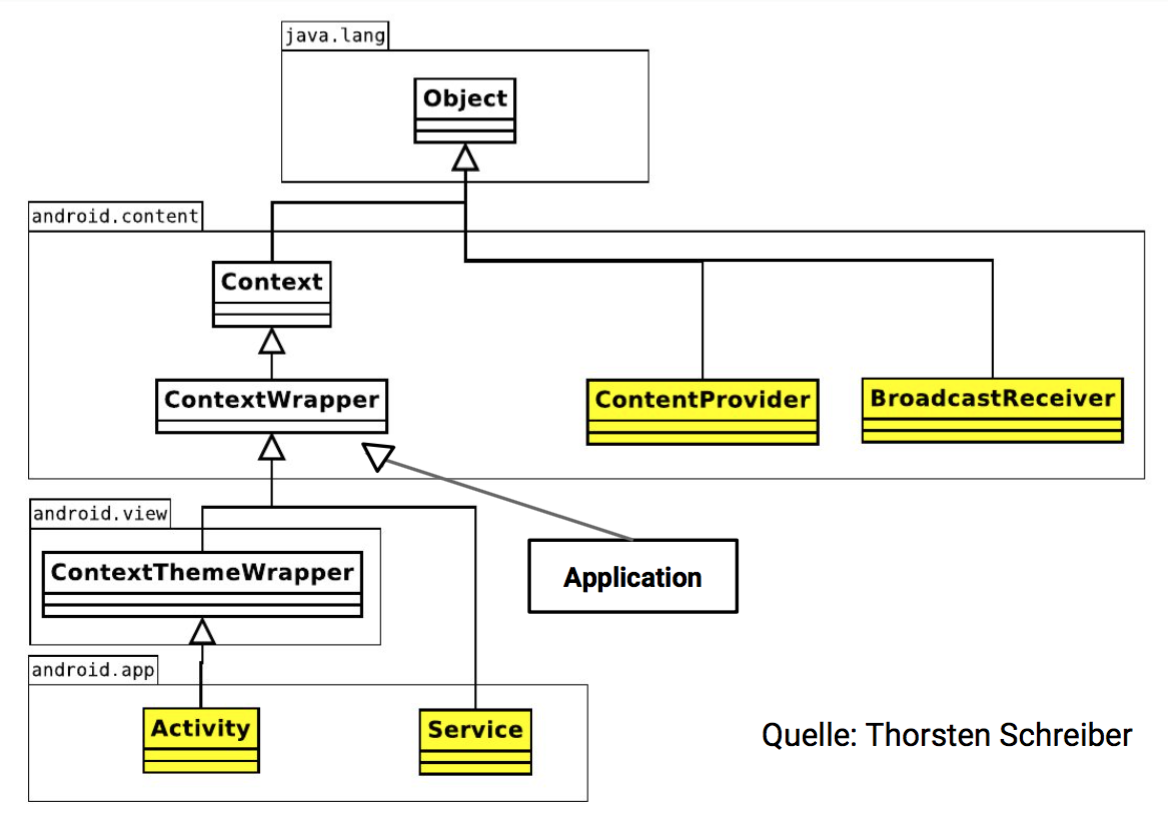
\includegraphics[scale=0.25]{komponentenEinerApp.png}
\paragraph{Context Klasse} Mit einer Context-Instanz kann man:
\begin{itemize}
\item Neue View erstellen (Kontext muss als Parameter mitgegeben werden)
\item Auf System-Service zugreifen (\code{context. getSystemService( LAYOUT\_INFLATER\_SERVICE)})
\item Die Applikationsinstanz erhalten
\item Neue Acativities starten (mittels Intent)
\item Preferences lesen und schreiben
\item Services starten
\end{itemize}
\subsection{Services}
Für Aufgaben die im Hintergrund ablaufen sollen oder deren Abarbeitung das UI zu lange blockieren würde, verwendet man Services. Diese haben folgende Eigenschaften:
\begin{itemize}
\item Kein UI
\item Können gestarted oder gebunden werden
\item Arbeiten im UI-Thread der Applikation, sind keine eigenen Threads
\item Müssen in der Manifest Datei deklariert werden
\end{itemize}
\paragraph{Deklaration} Wie Activities müssen auch Service-Komponenten im Manifest deklariert werden
\begin{lstlisting}[language=java]
<application>
  <service 
  android:name=".ExampleService"
  android:exported="false" />
</application>
\end{lstlisting}
Es gibt zwei verschiedene Arten von Services. Den \textbf{gebundenen} Service (Client-Server ähnliche Kommunikation über eine längere Zeitdauer) und den \textbf{gestarteten} Service (erledigen einmaliger Aufgaben).
\paragraph{Started Services} Ein Service wird mit \code{context.startService(intent)} gestartet. Der Service läuft im Hintergrund und wird nicht gestoppt, auch wenn der Anwender die App wechselt oder der startende Context zerstört wird (im Hintergrund meint nicht in einem eigenen Thread). Der Service soll sich selbst beenden, wenn der User die App wechselt. Grundsätzlich kann man sagen der Service entkoppelt Aufgaben vom Context, und der AsyncTask entkoppelt Aufgaben vom Main-Thread.
\paragraph{Bound Services} Ein Service wird mit \code{context.bindService(intent, ...)} gebunden. Der Service liefert ein Interface, das dem Client erlaubt, Methoden des Services aufzurufen. Es ist möglich, dass mehrere Clients gebunden sind. Wenn alle Clients \code{context.unbindService(...)} aufgerufen haben, wird der Service zerstört.
\paragraph{Lifecycle} Die Callbacks eines Services sind ähnlich wie die der Activitiy
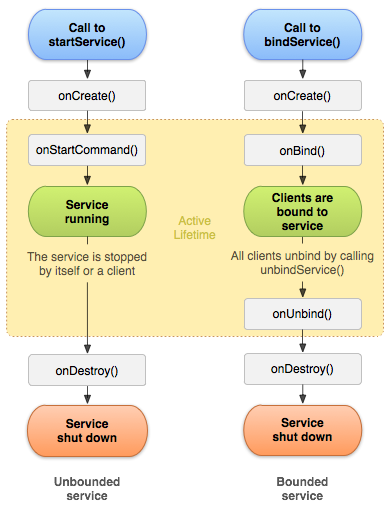
\includegraphics[scale=0.4]{service_lifecycle.png}
\paragraph{Started Service Starten} Der Service wird aus einer Activity gestartet.
\begin{lstlisting}[language=java]
Intent intent = new Intent(this, SimpleService.class);
this.startService(intent);
\end{lstlisting}
Dies ruft ggf \code{onCreate()} und anschliessen \code{onStartCommand()} im Service auf. Ohne Einstellung, findet keine Kommunikation zwischen Service und Acitivity statt.\\
Der Service kann mit \code{stopSelf()} gestoppt werden und sollte auch getan werden. Man kann den Service auch in der Acitivity stoppen, mittels \code{stopService()}.
\paragraph{Started Service IntentService} Der IntentService stellt einen Worker-Thread zur Verfügung. Er verwendet eine Queue, um Intents zwischenzuspeichern, welche sequentiell in \code{onHandleIntent()} abgearbeitet werden. Der Service wird gestoppt, nachdem alle Intents abgearbeitet wurden.
\begin{lstlisting}[language=java]
public class HelloIntentService extends IntentService {
  public HelloIntentService() {
  super("HelloIntentService");
  }
  @Override
  protected void onHandleIntent(Intent intent) { }
}
\end{lstlisting}

\paragraph{IntentService vs. AsyncTask}
Beide blockieren UI nicht. Beim \code{IntentService} ist die Chance höher, dass die Berechnung vollständig durchgeführt wird, da das System Prozesse (APK) mit Services höher gewichtet.

AsyncTask bietet Callback, IntentService einen Broadcast.

IntentService zum Wörter zählen (eigentliche Zählmethoden nicht gegeben)
\begin{lstlisting}[language=java]{language=java}
@Override
protected void onHandleIntent(Intent intent) {
  Log.d(FileActivity.DEBUG_TAG, "onHandleIntent()");

  // Intent auslesen
  Bundle bundle = intent.getExtras();
  if (bundle == null) {
    Log.d(FileActivity.DEBUG_TAG, "service bundle is null");
  }

  FileHolder fileHolder =
    (FileHolder) bundle.get(FileActivity.KEY_WORD_RESULT);
  if (fileHolder == null) {
    Log.d(FileActivity.DEBUG_TAG, "result is null");
  }

  // Resultat ermitteln
  String text = loadFile(fileHolder.id);
  List<WordCount> counters = analyzeText(text);
  WordCountResult result = 
    new WordCountResult(fileHolder, counters);

  // Activity starten
  Intent showResultIntent =
    new Intent(this, WordListActivity.class);
  Bundle bundle2 = new Bundle();
  bundle2.putSerializable(FileActivity.KEY_WORD_RESULT, result);
  showResultIntent.putExtras(bundle2);

  // Beim starten einer Activity ausserhalb einer Activity
  // müssen wir dieses Flag setzen:
  showResultIntent.addFlags(Intent.FLAG_ACTIVITY_NEW_TASK);

  startActivity(showResultIntent);
}
\end{lstlisting}

Der Service enthält keine Referenz an die aufrufende Activity. Um nun ein Resultat vom Service zu bekommen, kann man entweder einen Intent mit Resultat als Broadcast versenden, wo dann wiederum die Activity einen Broadcast-Receiver zur Verfügung stellen muss um den Intent zu empfangen. Oder man verwendet einen. \code{PendingIntent}.
\paragraph{Pending Intent} ist ein Objekt das einen Intent umhüllt (wrapped). Genauer ist es ein Token das man einer "{}Fremden App"{} übergiebt (e.g. \code{NotificationManager, AlarmManager} Home Screen \code{AppWidgetManager} oder 3rd Party Apps), welch die "Fremde App" berechtigt bestimmten Code auszuführen. \\
Wenn man der "{}fremden App"{} einen Intent übergibt, und diese App diesen Intent sendet/broadcastet, dann wird dieser Intent mit seinen eigenen Berechtigungen ausgeführt. Wenn man aber der "fremden App" einen PendingIntent übergibt werden die Berechtigungen der übergebenden App verwendet. Wird die Klasse, welche den PendingIntent erzeugt terminiert, bleibt der PendingIntent bestehen und kann von anderen Apps weiterverwendet werden. Intents behandelen spezifische Komponenten der App, genauso PendingIntents und nutzen dafür z.B. (\code{PendingIntent.getActivity() PendingIntent.getBroadcast() PendingIntent.getService()} \\
\textbf{Bsp. 1}: Intent erzeugen und wrappen, ausführen der Operation zugehörend zum PendingIntent (\code{send()})
\begin{lstlisting}[language=java]
// Explicit intent to wrap
Intent intent = new Intent(this, LoginActivity.class);

// Create pending intent and wrap our intent
PendingIntent pendingIntent = PendingIntent.getActivity(this, 1, intent, PendingIntent.FLAG_CANCEL_CURRENT);
try {
  // Perform the operation associated with our pendingIntent
  pendingIntent.send();
} catch (PendingIntent.CanceledException e) {
  e.printStackTrace();
}
\end{lstlisting}
\textbf{Besseres Bsp. 2}: Erzeugen, wrappen, starten mit AlarmManager nach 3 sec.
\begin{lstlisting}[language=java]
int seconds = 2;
// Create an intent that will be wrapped in PendingIntent
Intent intent = new Intent(this, MyReceiver.class);

// Create the pending intent and wrap our intent
PendingIntent pendingIntent = PendingIntent.getBroadcast(this, 1, intent, 0);

// Get the alarm manager service and schedule it to go off after 3s
AlarmManager alarmManager = (AlarmManager) getSystemService(ALARM_SERVICE);
alarmManager.set(AlarmManager.RTC_WAKEUP, System.currentTimeMillis() + (seconds * 1000), pendingIntent);

Toast.makeText(this, "Alarm set in " + seconds + " seconds", Toast.LENGTH_LONG).show();
\end{lstlisting}
Wenn man noch eine BroadcastReceiver onReceive() Methode hinzufügt, vibriert das Gerät für 2 sec. sobald ein Broadcast Event gesendet wurde.
\begin{lstlisting}[language=java]
@Override
public void onReceive(Context context, Intent intent) {
  // Vibrate for 2 seconds
  Vibrator vibrator = (Vibrator) context.getSystemService(Context.VIBRATOR_SERVICE);
  vibrator.vibrate(2000);
}
\end{lstlisting}
\paragraph{Bound Service} Der Bound Service funktioniert nach einem Client-Server Modell. Clients können Methoden eines Service aufrufen und die App kann die Funktionalität des Services andern Apps zur verfügugn stellen. Beim Aufruf von \code{BindService()} erhält der Client ein Interface um mit dem Service zu kommunizieren. Es ist möglich, dass mehrere Clients gleichzeitig gebunden sind. Nachdem alle Clients \code{unbindService()} aufgerufen haben, wird der Service beendet.
\paragraph{Bound Service: Server} Der Server muss von der Service Klasse und ein Binder implementieren.
\begin{lstlisting}[language=java]
public class LocalService extends Service {
  private final IBinder binder = new LocalBinder();
  public class LocalBinder extends Binder {
  LocalService getService() {
    return LoaclService.this;
  }
  }
  @Override
  public IBinder onBind(Intent intent) {
  return binder;
  }
  public int getRandomNumber() {
  return new Random.nextInt(100);
  }
}
\end{lstlisting}
\paragraph{Bound Service: Client} Ein Bound-Service liefert bei \code{onBind()} ein Interface vom Typ \code{IBinder}. Wenn der Service nur innerhalb der App und im gleichen Prozess arbeitet, sollte ein Binder als Interface geliefert werden. Clients rufen so die Methoden des Binders oder des Services auf.
\begin{lstlisting}[language=java]
Intent intent = new Intent(this, LocalService.class);
bindService(intent, connection, Context.BIND_AUTO_CREATE);
\end{lstlisting}
Der Aufruf von \code{bindService()} liefert nicht den \code{onBind()} Binder, sondern der Callback \code{onServiceConnected()} wird aufgerufen.
\begin{lstlisting}[language=java]
private ServiceConnection c = new ServiceConnection() {
  @Override
  public void onServiceConnected(ComponentName className, IBinder binder) {
  LocalService.LocalBinder myBinder = (...)binder;
  LocalService myService = myBinder.getService();
  int random = myService.getRandomNumer();
  }
  @Override
  public void onServiceDisconeccted(ComponentName name) {}
};
\end{lstlisting}
\paragraph{Bound Service: Messenger} Ein Messenger kann eingesetzt werden um prozessübergreifend Informationen auszutauschen. Der Service stellt dabei einen Handler zur Verfügung um Meldungen zu erhalten, welche er sequentiell abarbeitet. Für Rückgabewerte des Servers muss der Client seinerseits einen Messenger zur Verfügung stellen.
\subsection{Broadcast Receiver} Broadcasts sind Meldungen die als Intent verschickt werden. Die Action bestimmt den Ereignistyp. Eine Meldung enthält Informationen über ein bestimmtes Ereignis (SMS empfangen, System booted, Akku schwach etc.). Ein Broadcast Receiver kann registriert werden, um bestimmte Meldungen zu erhalten. Standartmeldungen des Systems umfassen unter anderem: \code{ACTION\_BOOT\_COMPLETED | ACTION\_POWER\_CONNECTED | ACTION\_POWER\_DISCONNECTED | ACTION\_BATTERY\_LOW | ACTION\_BATTERY\_OKAY}.
\paragraph{Broadcast Receiver: Registrieren} Man kann den Receiver entweder statisch in der Manifest Datei, dann ist der Receiver global in der App verfügbar (an keine Activity gebunden) und wird bei jeder Meldung neu instanziert. Dynamisch macht man das mit \code{context.registerReceiver()}. Dann wird der Receiver an die Activity gebunden und muss abgemeldet werden, wenn er nicht mehr benötigt wird.
\begin{lstlisting}[language=java][language=xml, caption="{}Statische Registration"]
<receiver android:name=".TimeChangedReceiver" >
  <intent-filter>
  <action android:name="android.intent.action.TIME_SET" />
  </intent-filter>
</receiver>
\end{lstlisting}
\begin{lstlisting}[language=java][caption="Dynamische Registration"]
LocalBroadcastManager lbm = LocalBroadcastManager.getInstance(getApplicationContext());
IntentFilter filter = new IntentFilter(Intent.ACTION_BOOT_COMPLETED);
MyBroadcastReceiver receiver = new MyBroadcastReceiver(this);
lbm.registerReceiver(receiver, filter);
\end{lstlisting}
\begin{lstlisting}[language=java][caption="Receiver abmelden"]
LocalBroadcastManager lbm = LocalBroadcastManager.getInstance(getApplicationContext());
lbm.unregisterReceiver(receiver);
\end{lstlisting}
\paragraph{Broadcast Receiver: Implementation} Die Implementation eines Receivers muss von der Klasse \code{BroadcastReceiver} ableiten. Die Methode \code{onReceive()} muss überschrieben werden um Meldungen zu erhalten und verarbeiten.
\begin{lstlisting}[language=java]
private class MyBroadcastReceiver extends BroadcastReceiver {
  public MyBroadcastReceiver(MainActivity activity) { }
  @Override
  public void onReceive(Context context, Intent intent){ }
}
\end{lstlisting}
\paragraph{Broadcast Receiver: Versenden} Der Broadcast Receiver kann auch Meldungen versenden (semantik?). Dies kann man mit der Methode \code{context.sendBroadcast(intent)}. Die Action im angegeben Intent definiert den Ereignistyp (Namensgebend und in der Action ist global, bei eigenen Actions, Name mit eigenem Namespace verwenden). Beim Intent können unter Extras zusätzliche Daten hinterlegt werden. Wenn man Meldungen nur im eigenen selben Prozess versenden möchte, sollte man den \code{LocalBroadcastManger verwenden}. So verlassen die Meldungen den Prozess nicht und andere Prozesse können unserer App keine Meldungen senden.
\subsection{Content Provider}
Der Content Provider stellt Daten prozessübergreifend zur Verfügung. Es ist ein Client-Server Modell. Der Provider Client und Provider kommunizieren über eine standartisierte Schnittstelle um Daten auszutauschen. Android stellt beispielsweise Kalender oder Kontakte über einen Content-Provider zur Verfügung.
\paragraph{Schnittstelle} eines Content Provider stellt in der Regel Daten zur Verfügung die in einer Tabelle in einer Datenbank abgelegt sind. Deshalb ähnelt die Schnittstelle stark der SQL Syntax.\\
\paragraph{Security} Der Content Provider kann Permissions setzte um den Zugriff auf die Daten einzuschränken. Die Clients müssen die erforderlichen Permissions im Manifest angeben.
\begin{lstlisting}[language=xml]
<uses-permission android:name="android.permission.READ_USER_DICTIONARY"/>
\end{lstlisting}
\paragraph{Content Provider: Client} Der ContentResolver stellt die Schnittstelle zur Verfügung. Die Tabelle des Content-Provider wird als URI angegeben: \code{content://user\_dictionary/words}.
\begin{lstlisting}[language=java]
Cursor cursor = getContentResolver().query(
  UserDictionary.Words.CONTENT_URI,
  mProjection,
  mSelectionClause,
  mSelectionArgs,
  mSortOrder);
int index = cursor.getColumnIndex(UserDictionary.Words.WORD);
while(cursor.moveToNext()){
  String word = cursor.getString(index);
}
\end{lstlisting}
\paragraph{Content Provider: Server} Der Einsatz eines eigenen Servers ist erforderlich wenn andere Apps strukturierte Daten oder Dateien zur Verfügung stehen sollen, oder wenn andere Apps die Möglichkeit haben sollen, Daten zu durchsuchen. Ein Provider kann Daten als Dateien oder strukturiert anbieten. Dateien werden im Internal Storage abgelegt, der Client erhält einen Handle um auf eine Datei zuzugreifen. Strukturierte Daten werden in der Regel in einer Datenbank abgelegt. Der ContentResolver hat gezeigt, dass das Prinzip von Tabellen mit Spalten und Reihen verwendet werden sollte. \textbf{Ein Content-Provider muss Thread-Save programmiert werden}.\\
Bei der Implementation muss man sich folgendes überlegen:
\begin{itemize}
\item Wie sollen Daten persistent gespeichert werden
\item Die Content-URI muss festgelegt werden
\item Die Klasse \code{ContentProvider} muss implementiert werden.
\item Eine Contract Klasse muss implementiert werden. Die Klasse enthält alle Bezeichner (Konstanten) die ein Client benötigt. Die Klasse muss zudem in den Applikationscode des Clients kopiert werden.
\item Permissions in der Manifest Datei müssen festgelegt werden
\end{itemize}
\section{Weiterführende Themen}
\subsection{Sensoren}
Bewegungs-, Umgebuns- und Lagesensoren.
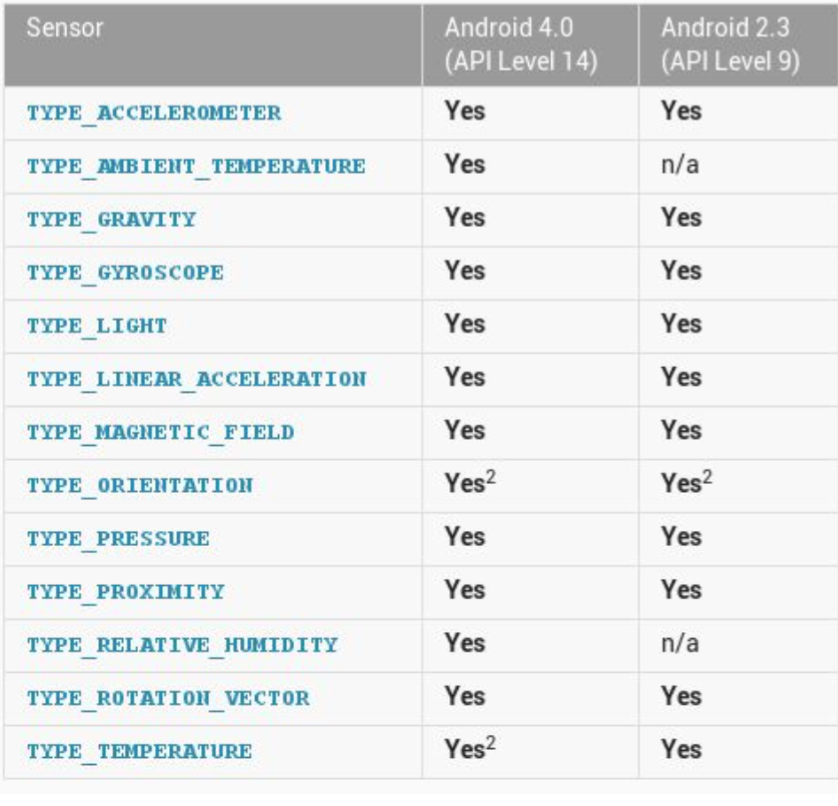
\includegraphics[scale=0.35]{sensors.png} \\
Für die Arbeit mit einem Sensor brauchen wir:
\begin{itemize}
\item \code{SensorManager} als Einstiegspunkt für die Sensoren
\item \code{Sensor} als Repräsentant für einen konkreten Sensor
\item \code{SensorEventListener} um Updates von Sensoren zu registrieren
\item \code{SensorEvent} um die Sensordaten auszulesen
\end{itemize}
Ein Sensor liefert uns nur Rohdaten! Je nach Sensor unterschiedlich zu interpretieren. Sensor Bsp.:
\begin{lstlisting}[language=java]
public class MainActivity extends AppCompatActivity implements SensorEventListener {
   private TextView textView;
   private SensorManager sensorManager;
   private Sensor lightSensor;
   @Override
   protected void onCreate(Bundle savedInstanceState) {
        // ...
        textView = (TextView) findViewById(R.id.textView);
        sensorManager = (SensorManager) getSystemService(Context.SENSOR_SERVICE);
       
        if (mSensorManager.getDefaultSensor(Sensor.TYPE_LIGHT) != null){
          // Success! There's a light sensor.
          lightSensor = sensorManager.getSensorList(Sensor.TYPE_LIGHT).get(0);
        }
        else {
          // Failure! No sensor.
        }
        
   }
   @Override
   protected void onResume() {
       super.onResume();
       //would return true if the sensor is supported and successfully enabled.
       sensorManager.registerListener(this, lightSensor, SensorManager.SENSOR_DELAY_NORMAL);
   }
   @Override
   protected void onPause() {
       super.onPause();
       sensorManager.unregisterListener(this);
   }
   @Override
   public void onSensorChanged(SensorEvent event) {
       textView.setText(String.format("Helligkeit: %.0f", event.values[0]));
   }
}
\end{lstlisting}
\subsection{View Injection}
Flexible Lösung wäre Service ausserhalb der Activity zu erstellen und dieser übergeben. Noch besser: Interface von LibraryService extrahieren und im Test durch einen Fake-Server ersetzen. Die Klasse erstellt seine Dependencies also nicht selbst, stattdessen werden diese injiziert (injected). \\
Einfache Lösung: Konstruktor mit Parametern und final-Attributen. Stellt sicher das Klasse vollständig initialisiert wurde. \\
Weniger Schön: Setter Methoden. Benutzer muss aufpassen das alle aufruft. \\
Dagger Tool verwenden: \textbf{Modul} instanziert unsere Klasse(z.B. LibraryService) die wir injecten wollen. \textbf{Komponente} fasst Module zusammen und ist zuständig für die Injection. Eine Klasse lässt sich über die Komponenten ihre Abhängigkeiten injecten.
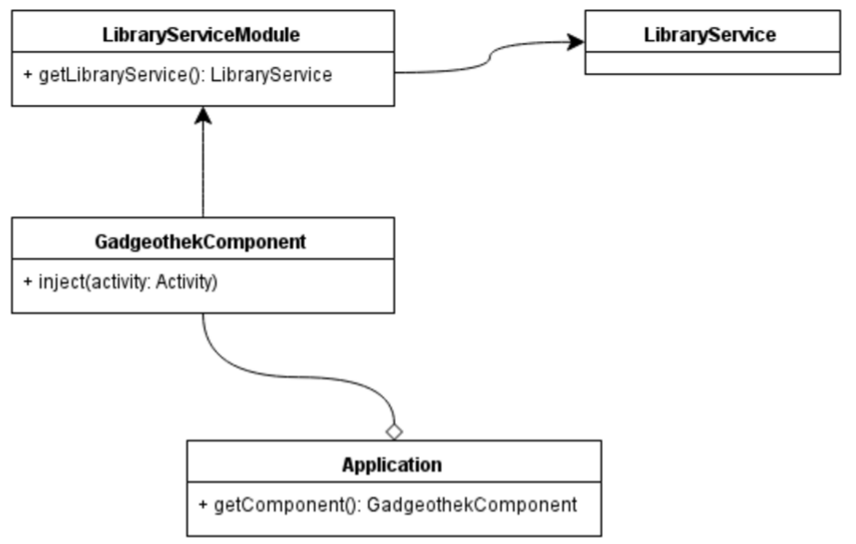
\includegraphics[scale=0.35]{Injection1.png} \\
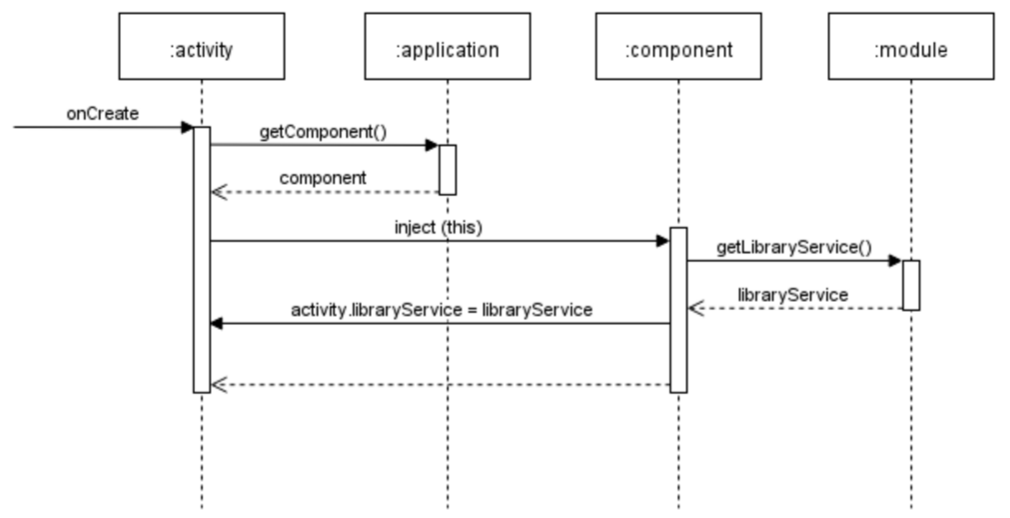
\includegraphics[scale=0.35]{Injection2.png}
\begin{lstlisting}[language=java]
@Module
public class LibraryServiceModule {
   @Provides
   @Singleton
   public LibraryService getLibraryService() {
     return new LibraryService();
   }
}


@Singleton
@Component(modules = {LibraryServiceModule.class})
public interface GadgeothekComponent {
   void inject(GadgeothekActivity activity);
}
\end{lstlisting}
\begin{lstlisting}[language=java]
public class Application extends android.app.Application {
   GadgeothekComponent component;

   public void onCreate() {
     component = DaggerGadgeothekComponent.builder().build();
   }

   public GadgeothekComponent getComponent() {  return component;  }
}


public class GadgeothekActivity extends AppCompatActivity {

   @Inject
   LibraryService libraryService;

   @Override
   protected void onCreate(Bundle savedInstanceState) {
   ...
   ((Application) getApplication()).getComponent().inject(this);
\end{lstlisting}
Lohnt sich Dependency Injection? \\
Vorteile:
\begin{itemize}
\item keine statischen Methoden mehr
\item zentrale Konfiguration in Modul und Komponente
\item Einfache Testbarkeit: Modul oder Applikation austauschen
\end{itemize}
Nachteile:
\begin{itemize}
\item Nicht unbedingt weniger Schreibaufwand bei kleinen Projekten
\item Braucht Tests: bei einer Fehlkonfiguration drohen NullPointerException
\item Spaghetticode?
\end{itemize}
\subsection{Data Binding}
\begin{itemize}
\item erspart Tipparbeit
\item in XML direkt auf Objekte zugreifen (Bsp. \code{onClick})
\item Optimal: GUI aktualisiert sich selbst, sobald Objekt sich ändert
\begin{itemize}
\item XML-Layout als Observer
\item Einfache Logik (x ? y : z) direkt im XML
\end{itemize}
\item noch Beta
\end{itemize}
\begin{lstlisting}[language=java]
public class User {
   public String firstName;
   public String lastName;

   public User(String firstName, String lastName) {
     this.firstName = firstName;
     this.lastName = lastName;
   }
}
\end{lstlisting}
\begin{lstlisting}[language=java]
<layout xmlns:android="http://schemas.android.com/apk/res/android">
   <data >
     <variable name="user" type="ch.hsr.mge.databindingdemo.User"/>
   </data>
   <RelativeLayout
     ... >

     <TextView android:text="@{user.firstName}" ... />

     <TextView android:text="@{user.lastName}"  ... />
   </RelativeLayout>
</layout>
\end{lstlisting}
Expression Language unterstützt fast alle Java Expressions (Keine Statements Deklarationen, Loops, kein new, this und super)
\begin{lstlisting}[language=java]
android:text="@{String.valueOf(index + 1)}"
android:visibility="@{age < 13 ? View.GONE : View.VISIBLE}"
android:transitionName='@{"image_" + id}'
\end{lstlisting}
\begin{lstlisting}[language=java]
public class MainActivity extends AppCompatActivity {

   @Override
   protected void onCreate(Bundle savedInstanceState) {
     super.onCreate(savedInstanceState);

     ActivityMainBinding binding = 
       DataBindingUtil.setContentView(this, R.layout.activity_main);

     User user = new User("Mirko", "Stocker");
     binding.setUser(user);
   }
}
\end{lstlisting}
Neben Properties können auch Events gebunden werden
\begin{lstlisting}[language=java]
<Button
   android:text="Save"
   android:onClick="@{controller.onButtonSaveClicked}"/>
   <EditText
   android:text="@{user.lastName}"
   android:addTextChangedListener="@{user.lastNameWatcher}" />
\end{lstlisting}
Was wenn gebundene Objekt sich ändert?
\begin{lstlisting}[language=java]
public class User {
   public String lastName;
   public boolean isDirty;
  
   public TextWatcher lastNameWatcher = new TextWatcher() {
     @Override
     public void beforeTextChanged(CharSequence s, int start, int count, int after) { }

     @Override
     public void onTextChanged(CharSequence s, int start, int before, int count) {
       lastName = s.toString();
     }

     @Override public void afterTextChanged(Editable s) { }
   };
}
\end{lstlisting}
Um Daten aus gebundenen Objekten in der View zu aktualisieren benötigen wir wieder das Observer-Pattern. \textbf{View} observiert das gebundene Objekt. \textbf{Objekt} ist observable. Um unser Objekt observable zu machen müssen wir \code{ObservableFields} verwenden.
\begin{lstlisting}[language=java]
public class User {
   public ObservableField<String> firstName = new ObservableField<>();
   public ObservableField<String> lastName  = new ObservableField<>();

   public TextWatcher lastNameWatcher = new TextWatcher() {
   ...
      if (!Objects.equals(lastName.get(), s.toString())) {
        lastName.set(s.toString());
      }
   }
};
\end{lstlisting}

\subsection{Gradle}

\begin{lstlisting}
// build.gradle APP
apply plugin: 'com.android.application'

android {
    compileSdkVersion 26
    buildToolsVersion '26.0.2'
    defaultConfig {
        applicationId "io.teiler.android"
        minSdkVersion 23
        targetSdkVersion 26
        versionCode 1
        versionName "1.0"
        testInstrumentationRunner "android.support.test.runner.AndroidJUnitRunner"
    }
    buildTypes {
        release {
            minifyEnabled false
            proguardFiles getDefaultProguardFile('proguard-android.txt'), 'proguard-rules.pro'
        }
    }
}

repositories { jcenter() }
ext { materialSpinnerVersion = "1.2.1" }
dependencies {}

// build.gradle ROOT
// Top-level build file where you can add configuration options common to all sub-projects/modules.

buildscript {
    ext.kotlin_version = '1.1.51'
    repositories {
        google()
        jcenter()
    }
    dependencies {
        classpath 'com.android.tools.build:gradle:3.0.1'
        classpath ...
    }
}

allprojects {
    repositories {
        google()
        jcenter()
    }
}
\end{lstlisting}

\subsection{RecyclerView}

\begin{lstlisting}[language=java]
public class MyAdapter extends RecyclerView.Adapter < ViewHolder > {
 private ArrayList < Person > dataset;
 public MyAdapter(ArrayList < Person > persons) {
  dataset = persons;
 }
 @Override
 public ViewHolder onCreateViewHolder(ViewGroup parent, int viewType) {
  LayoutInflater layoutInflater = LayoutInflater.from(parent.getContext());
  View v = layoutInflater.inflate(R.layout.rowlayout, parent, false);
  TextView firstName = (TextView) v.findViewById(R.id.firstName);
  TextView lastName = (TextView) v.findViewById(R.id.lastName);
  ViewHolder viewHolder = new ViewHolder(v, firstName, lastName);
  return viewHolder;
 }
 @Override
 public void onBindViewHolder(ViewHolder holder, int position) {
  final Person person = dataset.get(position);
  holder.firstName.setText(person.getFirstname());
  holder.lastName.setText(person.getLastname());
 }
 @Override
 public int getItemCount() {
  return dataset.size();
 }
}
public class ViewHolder extends RecyclerView.ViewHolder {
 final TextView firstName;
 final TextView lastName;
 public ViewHolder(View v, TextView firstName, TextView lastName) {
  super(v);
  this.firstName = firstName;
  this.lastName = lastName;
 }
}
\end{lstlisting}

\end{multicols*}
\end{document}
